\subsection{Figuras}

\begin{frame}
\epigraph{I call our world Flatland, not because we call it so, 
but to make its nature clearer to you, my happy readers, 
who are privileged to live in space.}{Edwin A. Abbott, Flatland: A Romance of Many Dimensions}
\end{frame}


\begin{frame}
\frametitle{Figuras}
Figuras possuem uma grande potencial para levar informação de forma simples ao leitor.
Podem evidenciar padrões, tendências e anomalias, constâncias ou variações. 
Devem ser utilizadas com parcimônia e muito bem elaboradas.

\vspace{3ex}
Figuras são elementos flutuantes e que devem ser capazes de passar uma mensagem sozinhas.
\end{frame}


\begin{frame}
\frametitle{xkcd}
\begin{figure}[h]
\centering
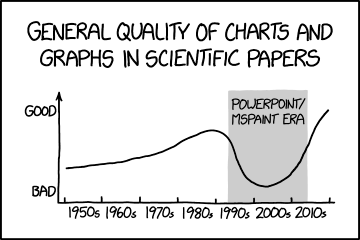
\includegraphics[width=0.6\textwidth,height=0.6\textheight,keepaspectratio]{figures/scientific_paper_graph_quality.png}
\caption{Scientific Paper Graph Quality (\url{https://xkcd.com/1945/}).}
\label{fig-scientific_paper_graph_quality}
\end{figure}
\end{frame}

\begin{frame}
\frametitle{Eventos na história da visualização de dados}
\begin{figure}[h]
\centering
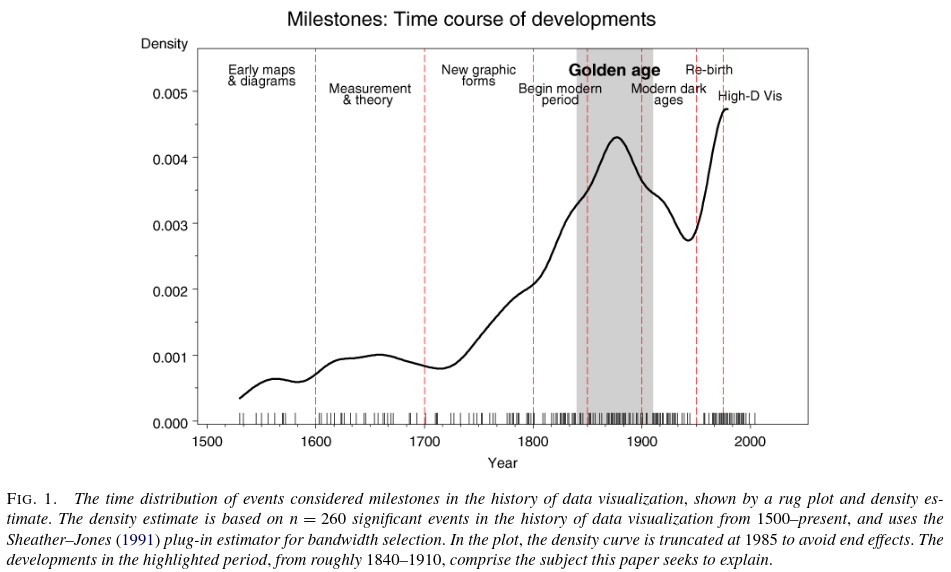
\includegraphics[width=0.8\textwidth,height=0.8\textheight,keepaspectratio]{figures/hist_data_visualization.png}
\caption{Retirada de \textcite{Friendly2008}.}
\label{fig-hist_data_visualization}
\end{figure}
\end{frame}


\begin{frame}
\frametitle{Figuras}

Florence Nightingale liderou uma pequena equipe de enfermeiras a Istambul em
1854 para ajudar no cuidado dos soldados britânicos que lutaram na guerra da
Crimeia. Seus gráficos convenceram os grandes e os bons de que as mortes devido
à sujeira e ao saneamento deficiente poderiam ser evitadas - salvando inúmeras
vidas.

\vspace{2ex}
\fullcite{harford_florence}

\vspace{1ex}
\hrefcolor{https://99percentinvisible.org/episode/florence-nightingale-data-viz-pioneer/}{Florence Nightingale: Data Viz Pioneer, 99percentinvisible.org}

\hrefcolor{https://en.wikipedia.org/wiki/Florence_Nightingale}{Florence Nightingale, Wikipedia}

\hrefcolor{https://www.youtube.com/watch?v=VTdVPNvwULM}{Nightingale Diagrams, Numberphile}

\hrefcolor{https://www.youtube.com/watch?v=sNppKQh0xPo}{What would Florence Nightingale make of big data?, BBC Ideas}
\end{frame}
% Coxcomb plots and 'spiecharts' in R
% https://rpubs.com/RobinLovelace/11641

\begin{frame}
\frametitle{Florence Nightingale}
\begin{figure}[h]
 \centering
 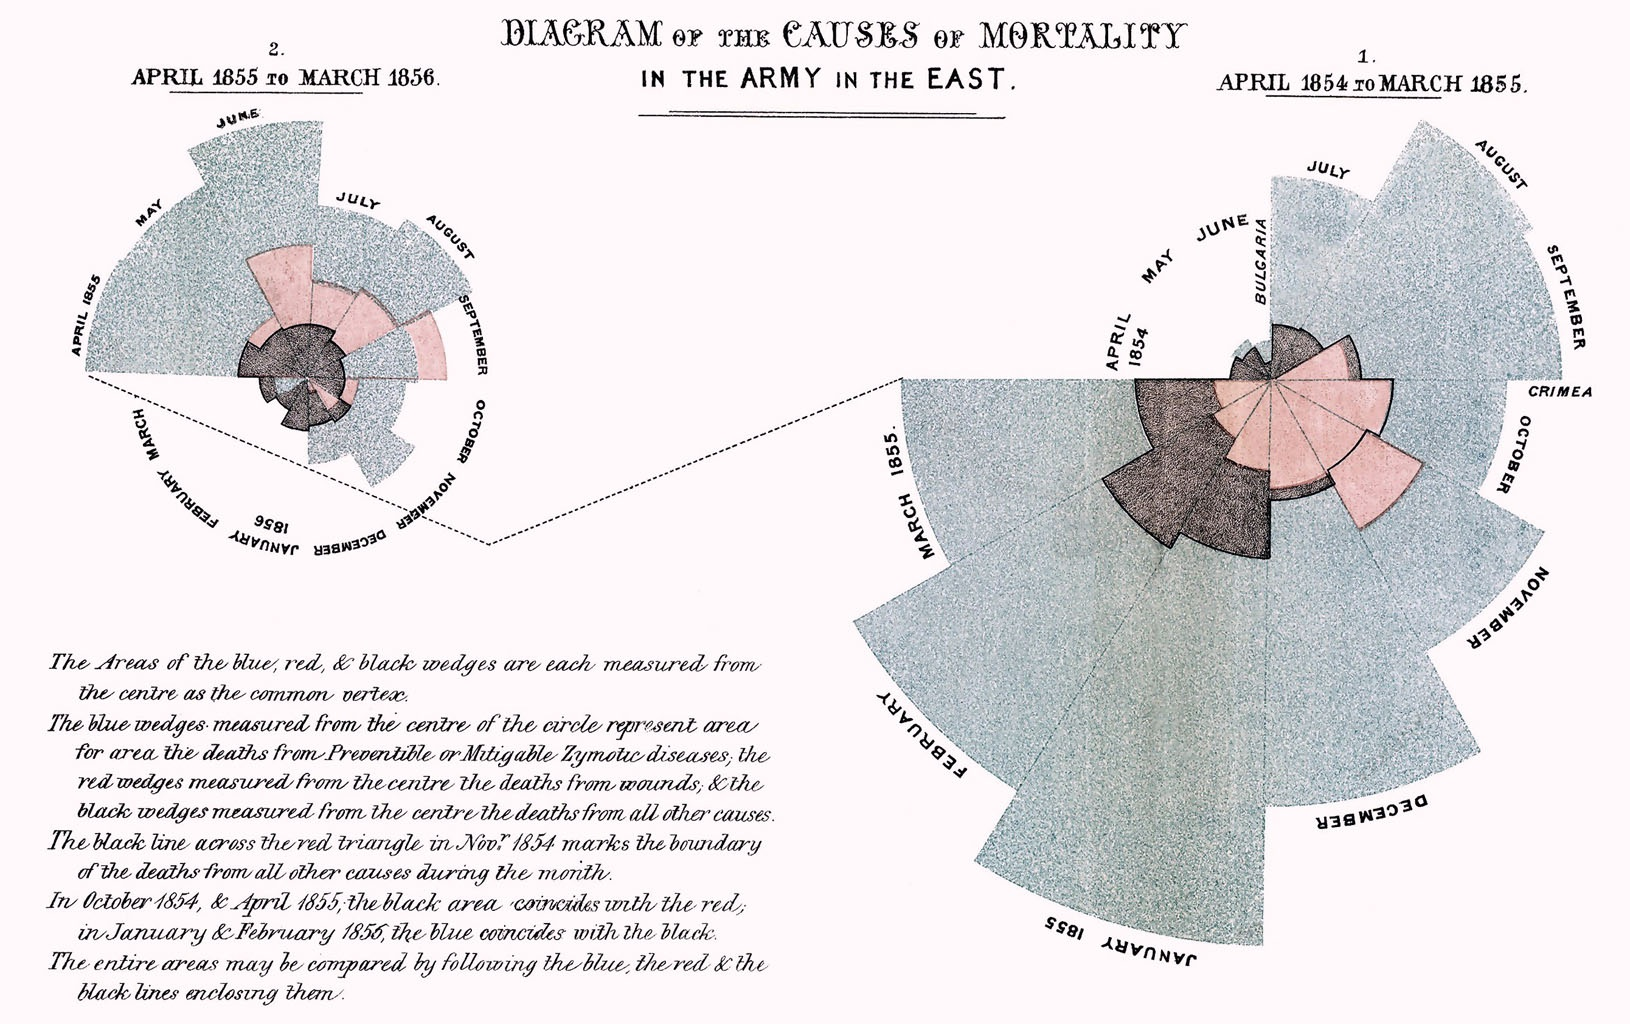
\includegraphics[width=0.8\textwidth,height=0.75\textheight,keepaspectratio]{figures/nightingale-mortality.jpg}
 \caption{Diagrama de mortalidade feito por Florence Nightingale.}
 \label{fig-nightingale-mortality}
\end{figure}
\end{frame}
\note{
O gráfico proposto por Florence Nightingale evidencia as mortes pelas áreas, sendo
dividas por três causas: doenças infectocontagiosas (azul), ferimentos (vermelho) e outras (preto).
O gráfico da direito apresenta o período durante a guerra antes da adoção de medidas sanitárias
e o gráfico da esquerda evidencia o período após a adoções de medidas sanitárias. 
O tempo é visto no sentido horário e a posição no gráfico facilita a comparação dos
meses em anos diferentes.
}






\begin{frame}[allowframebreaks]
\frametitle{Exemplo 1 - \emph{Storytelling with Data}}
\begin{figure}[h]
 \centering
 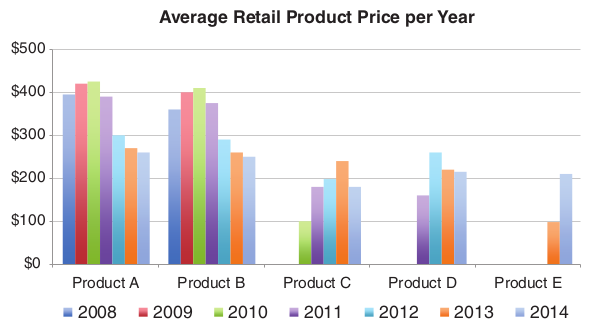
\includegraphics[width=0.8\textwidth,height=0.6\textheight,keepaspectratio]{figures/storytelling_data_ex01a.png}
 \caption{Preço médio de venda de produtos ao longo dos anos \cite{knaflic_storytelling_2015}.}
 \label{fig-storytelling_data_ex01a}
\end{figure}
\framebreak
\begin{figure}[h]
 \centering
 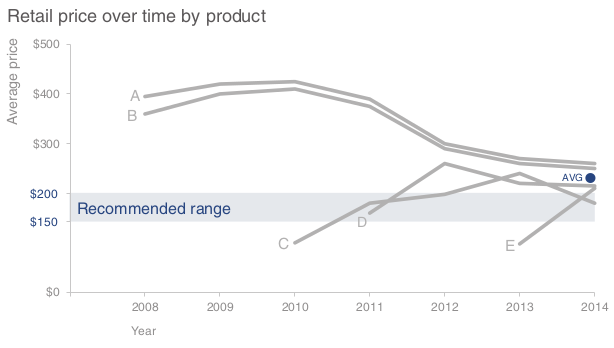
\includegraphics[width=0.8\textwidth,height=0.7\textheight,keepaspectratio]{figures/storytelling_data_ex01b.png}
 \caption{Preço médio de venda de produtos ao longo dos anos \cite{knaflic_storytelling_2015}.}
 \label{fig-storytelling_data_ex01b}
\end{figure}
\end{frame}


\begin{frame}[allowframebreaks=1]
\frametitle{Exemplo 2 - \emph{Storytelling with Data}}
\begin{figure}[h]
 \centering
 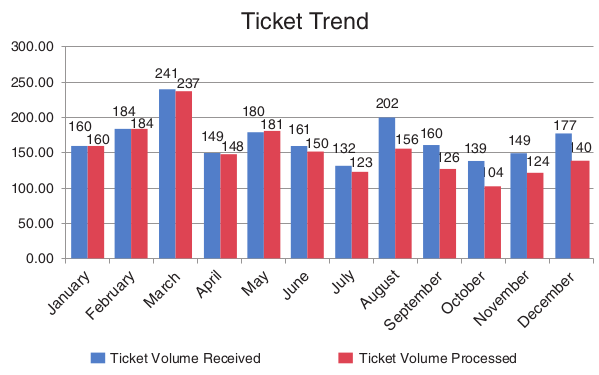
\includegraphics[width=0.8\textwidth,height=0.6\textheight,keepaspectratio]{figures/storytelling_data_ex02a.png}
 \caption{Volume de tickes recebidos e processados. \cite{knaflic_storytelling_2015}.}
 \label{fig-storytelling_data_ex02a}
\end{figure}
\framebreak
\begin{figure}[h]
 \centering
 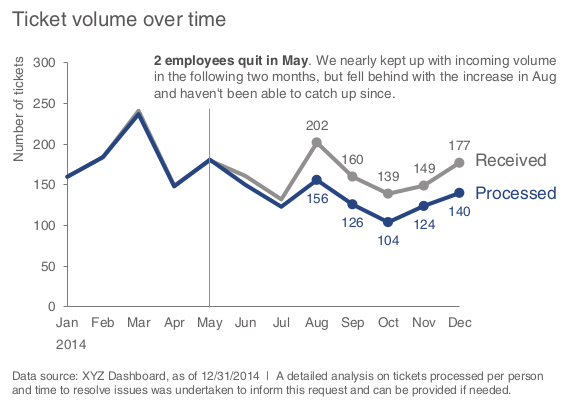
\includegraphics[width=0.8\textwidth,height=0.7\textheight,keepaspectratio]{figures/storytelling_data_ex02b.png}
 \caption{Volume de tickes recebidos vs. processados. O descolamento evidencia a necessidade de contratação. \cite{knaflic_storytelling_2015}.}
 \label{fig-storytelling_data_ex02b}
\end{figure}
\end{frame}

\begin{frame}[allowframebreaks=1]
\frametitle{Exemplo 3 - \emph{Storytelling with Data}}
\begin{figure}[h]
 \centering
 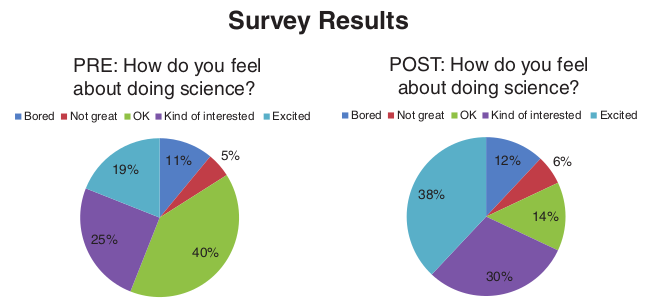
\includegraphics[width=0.8\textwidth,height=0.6\textheight,keepaspectratio]{figures/storytelling_data_ex03a.png}
 \caption{Resultado da pesquisa de opinião sobre ciências. \cite{knaflic_storytelling_2015}.}
 \label{fig-storytelling_data_ex03a}
\end{figure}
\framebreak
\begin{figure}[h]
 \centering
 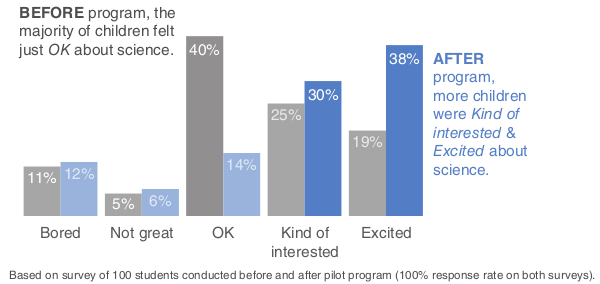
\includegraphics[width=0.7\textwidth,height=0.6\textheight,keepaspectratio]{figures/storytelling_data_ex03b.png}
 \caption{Resultado da pesquisa de opinião sobre ciências. \cite{knaflic_storytelling_2015}.}
 \label{fig-storytelling_data_ex03b}
\end{figure}
\end{frame}


\begin{frame}[allowframebreaks,fragile]
\frametitle{Limitações de alguns gráficos}

\begin{lstlisting}[language=Octave, label=lst-pie-ex, caption={Exemplo de limitações do gráficos.}, postbreak=\mbox{$\hookrightarrow$\space}, basicstyle=\fontsize{8}{10}\selectfont\ttfamily]
x = [0.07 0.12 0.08 0.13 0.075 0.126 0.083 0.135 0.063 0.118]; 
pie(x,strcat('item',strsplit(num2str(1:length(x)))));
print -dsvg piex.svg

lbs=strcat('item',strsplit(num2str(1:length(x))));
[_,idx]=sort(x);
pie(x(idx),lbs(idx)); 

plot(x,'ok','markerfacecolor','k')
set(gca,'Visible','off')
axes('Position',get(gca,'Position'),'XAxisLocation','bottom','YAxisLocation','left', 'Color','none','XTickLabel',get(gca,'XTickLabel'),'YTickLabel',get(gca,'YTickLabel'),'XColor','k','YColor','k','LineWidth',1,'TickDir','out');
print -dsvg piex-dots.svg

plot(x(idx),'ok','markerfacecolor','k');
set(gca,'xtick',[1:length(x)]); set(gca,'xticklabel',lbs(idx));

plot(x(idx),'ok','markerfacecolor','k');
set(gca,'Visible','off')
axes('Position',get(gca,'Position'),'XAxisLocation','bottom','YAxisLocation','left', 'Color','none','XTick',linspace(1/(length(x)),1,length(x)),'XTickLabel',lbs(idx),'YTickLabel',get(gca,'YTickLabel'),'XColor','k','YColor','k','LineWidth',1,'TickDir','out');
print -dsvg piex-dots-order.svg

pie3([0.2 0.2 0.2 0.4],{'','','',''}); view (0,12);
print -dsvg pie3d.svg
\end{lstlisting}

\begin{figure}[h]
 \centering
  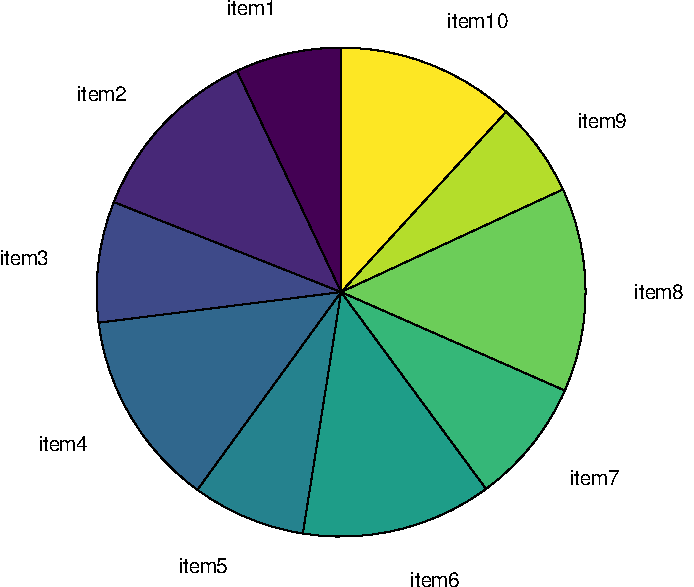
\includegraphics[width=0.6\textwidth,height=0.6\textheight,keepaspectratio]{figures/piex.pdf}
 \caption{Gráfico pizza gerado pelo código na lista \ref{lst-pie-ex}. Qual item é maior? e menor?}
 \label{fig-piex}
\end{figure}


\begin{figure}[h]
 \centering
  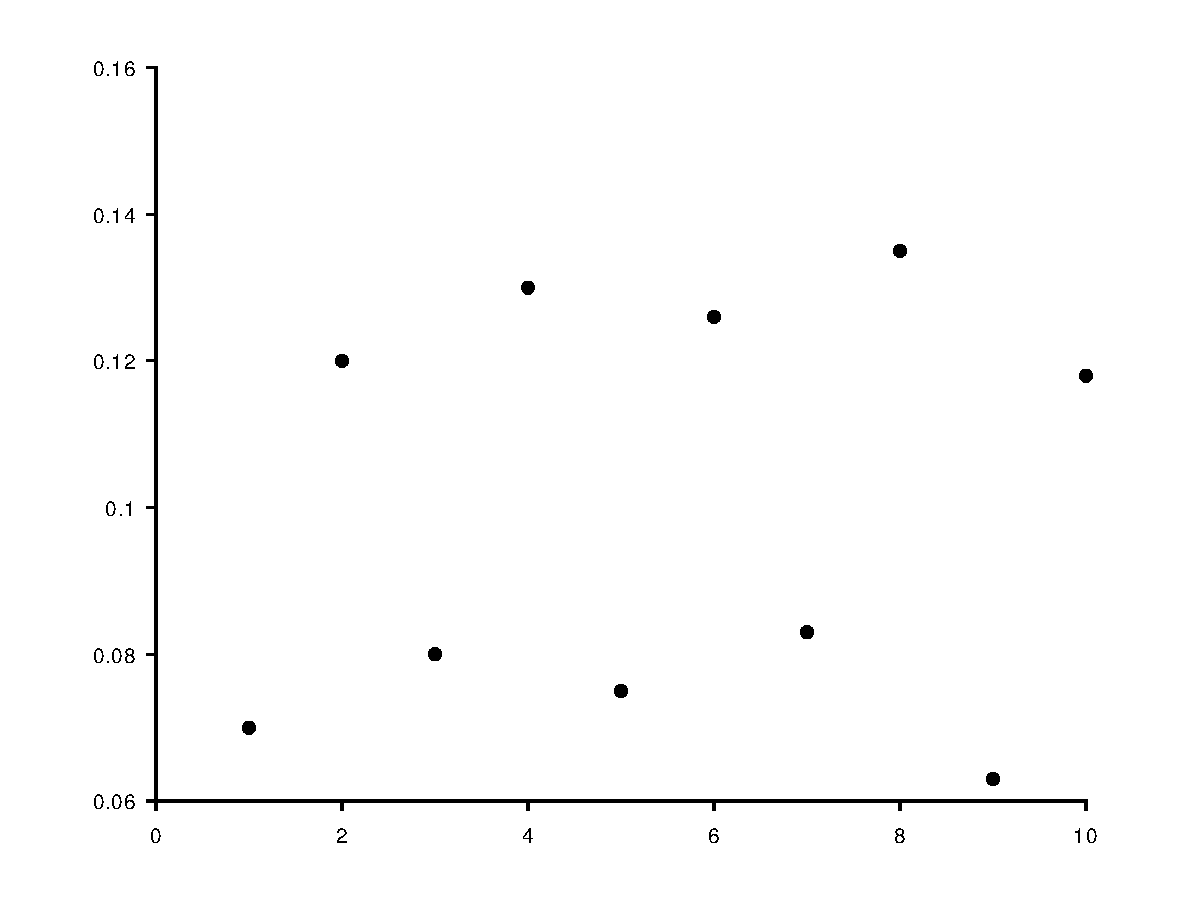
\includegraphics[width=0.8\textwidth,height=0.7\textheight,keepaspectratio]{figures/piex-dots.pdf}
 \caption{Gráfico de pontos gerado pelo código na lista \ref{lst-pie-ex}. É possível distinguir dois grupos.}
 \label{fig-piex2}
\end{figure}

\begin{figure}[h]
 \centering
  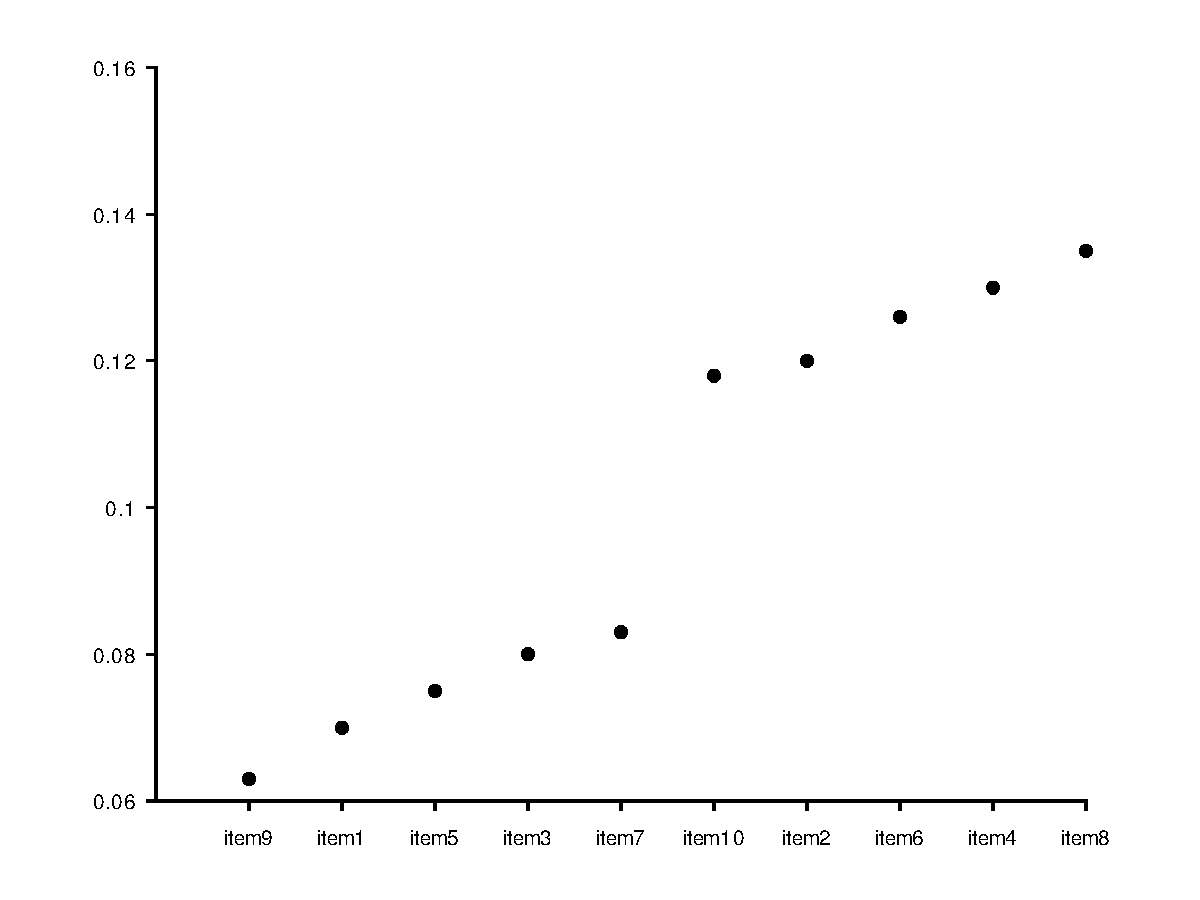
\includegraphics[width=0.8\textwidth,height=0.65\textheight,keepaspectratio]{figures/piex-dots-order.pdf}
 \caption{Gráfico de pontos gerado pelo código na lista \ref{lst-pie-ex}. É possível distinguir dois grupos e verificar a ordem de valores dos itens.}
 \label{fig-piex3}
\end{figure}

\begin{quote}
"Pie charts have severe perceptual problems. Experiments in graphical perception have shown
that compared with dot charts, they convey information far
less reliably. But if you want to display some data, and perceiving the information is not so important, then a pie chart
is fine." \cite{becker1996}
\end{quote}

\begin{quote}
"dumb pie chart; the only worse design than a pie chart is several of them,
for then the viewer is asked to compare quantities located in
spatial disarray both within and between pies. ... Given their
low data-density and failure to order numbers along a visual
dimension, pie charts should never be used." \cite{tufte_visual_1999}
\end{quote}

\framebreak

\begin{figure}[h]
 \centering
  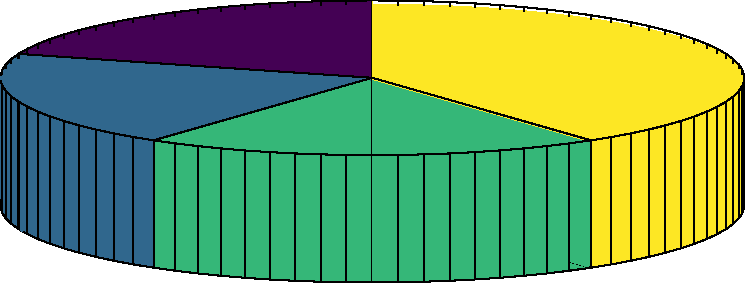
\includegraphics[width=0.7\textwidth,height=0.5\textheight,keepaspectratio]{figures/pie3d.pdf}
 \caption{Nada é tão ruim que não possa piorar.}
 \label{fig-pie3d}
\end{figure}

\framebreak

\begin{figure}[h]
 \centering
  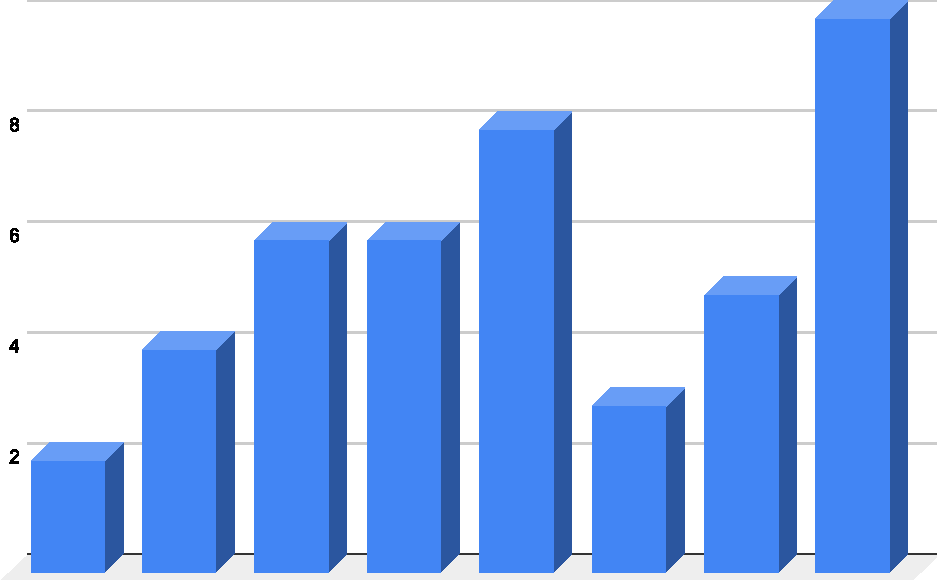
\includegraphics[width=0.7\textwidth,height=0.5\textheight,keepaspectratio]{figures/3dbars.pdf}
 \caption{Evite gráficos com 3D desnecessários.}
 \label{fig-3dbars}
\end{figure}

\end{frame}


\begin{frame}[allowframebreaks]
\frametitle{Playfair's Balance-of-Trade}

\begin{figure}[h]
 \centering
  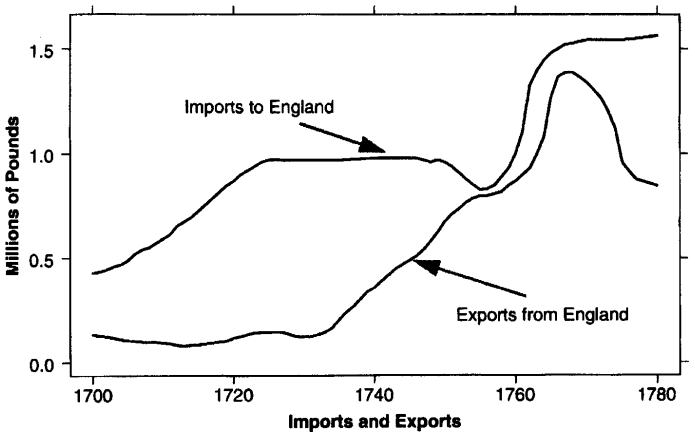
\includegraphics[width=0.7\textwidth,height=0.6\textheight,keepaspectratio]{figures/imports-exports.png}
 \caption{Balanço de comércio.}
 \label{fig-importex1}
\end{figure}

\framebreak

\begin{figure}[h]
 \centering
  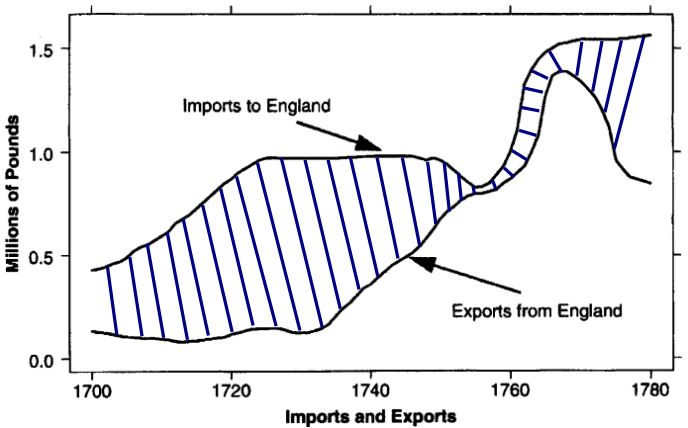
\includegraphics[width=0.7\textwidth,height=0.6\textheight,keepaspectratio]{figures/imports-exports_a.png}
 \caption{Balanço de comércio.}
 \label{fig-importex1a}
\end{figure}

\framebreak

\begin{figure}[h]
 \centering
  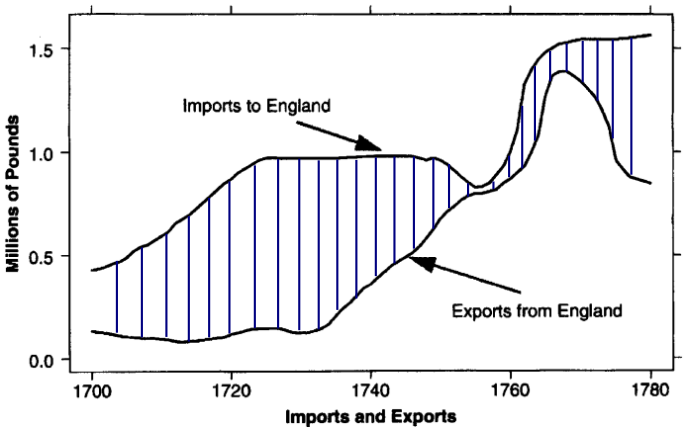
\includegraphics[width=0.7\textwidth,height=0.6\textheight,keepaspectratio]{figures/imports-exports_b.png}
 \caption{Balanço de comércio.}
 \label{fig-importex1b}
\end{figure}

\framebreak

\begin{figure}[h]
 \centering
  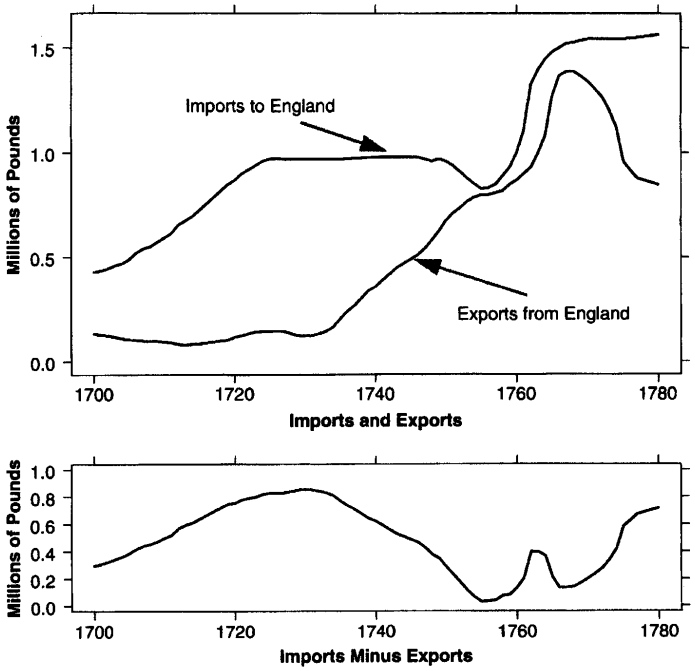
\includegraphics[width=0.7\textwidth,height=0.9\textheight,keepaspectratio]{figures/imports-exports2.png}
 \caption{Balanço de comércio.}
 \label{fig-importex2}
\end{figure}

\end{frame}




\begin{frame}[allowframebreaks,fragile]
\frametitle{Limitações de alguns gráficos}

\begin{lstlisting}[language=Octave, label=lst-y1y2, caption={Onde as curvas $y_1$ e $y_2$ estão mais próximas e mais distantes?}, postbreak=\mbox{$\hookrightarrow$\space}, basicstyle=\fontsize{8}{10}\selectfont\ttfamily]
x = [0.5:0.125:3];
y1 = 1./x.^2; y2 = y1 + 0.6;
plot(x,y1,'-',x,y2,'--'); legend('y_1','y_2');
print -dsvg curvesy1y2.svg
\end{lstlisting}

\begin{figure}[h]
 \centering
  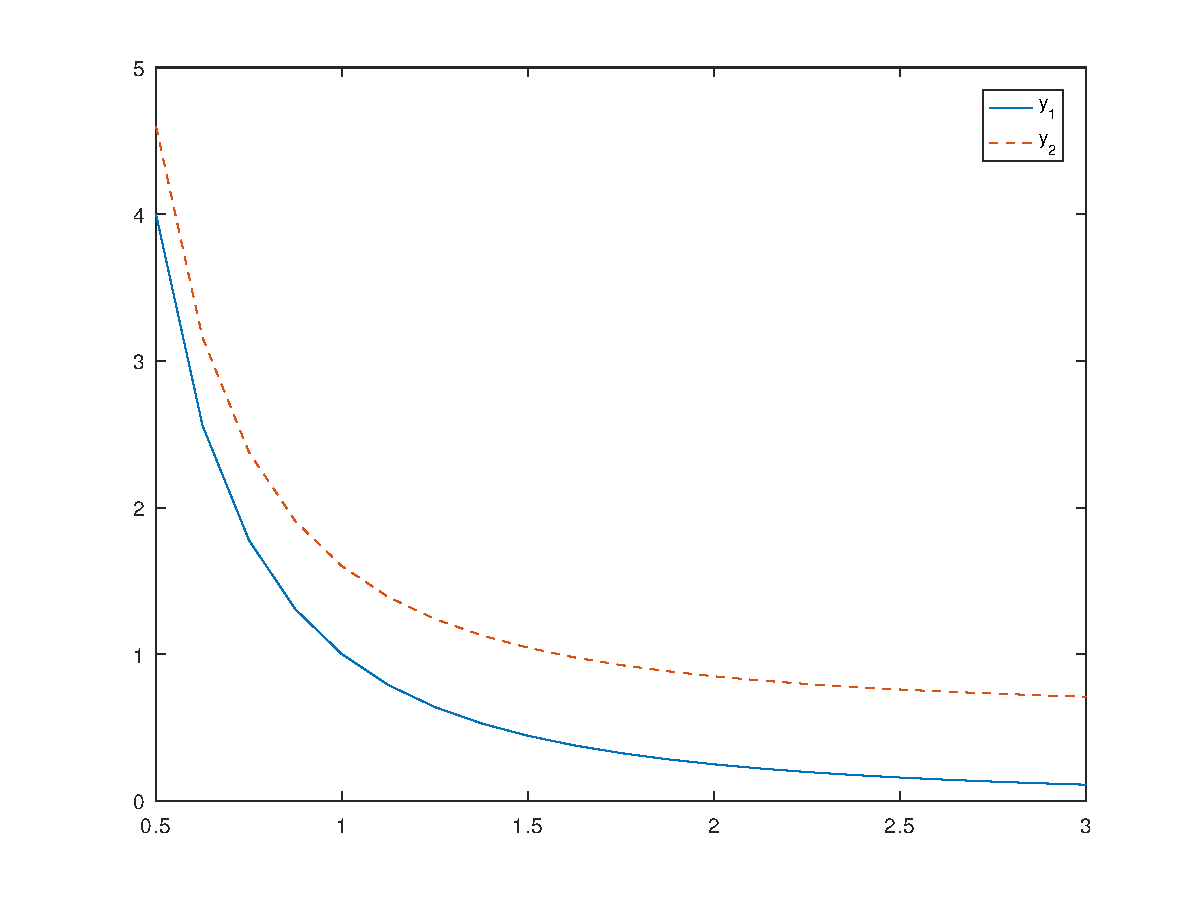
\includegraphics[width=0.7\textwidth,height=0.9\textheight,keepaspectratio]{figures/curvesy1y2.pdf}
 \caption{Diferença entre as curvas.}
 \label{fig-curvesy1y2}
\end{figure}

\end{frame}


\begin{frame}[allowframebreaks,fragile]
\frametitle{Limitações de alguns gráficos}
\begin{lstlisting}[language=Octave, label=lst-y1y2, caption={Onde as curvas $y_1$ e $y_2$ estão mais próximas e mais distantes?}, postbreak=\mbox{$\hookrightarrow$\space}, basicstyle=\fontsize{8}{10}\selectfont\ttfamily]
system('wget https://gist.githubusercontent.com/curran/13d30e855d48cdd6f22acdf0afe27286/raw/0635f14817ec634833bb904a47594cc2f5f9dbf8/worldcities_clean.csv -O /tmp/worldcities.csv')
X = csvread ('/tmp/worldcities.csv');
top100 = X(2:104,5);
id=find(top100==0);
top100(id)=[];
figure; hold on; for i=1:10:100, drawCircle(i-1,top100(i)/top100(end),top100(i)/top100(end)); end; plot([0:99],top100./top100(end),'k-'); hold off; daspect([1 1 1]);
\end{lstlisting}

\begin{figure}[h]
 \centering
  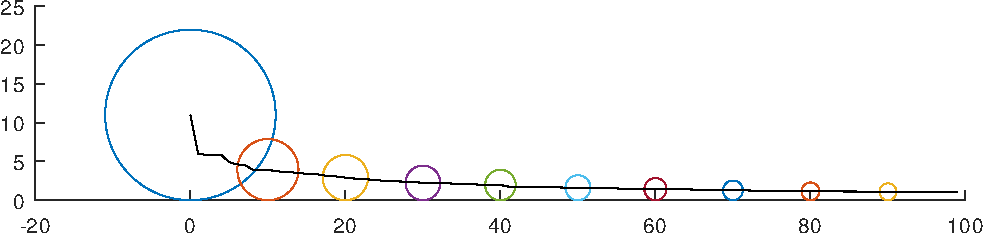
\includegraphics[width=\textwidth,height=0.5\textheight,keepaspectratio]{figures/citiespop.pdf}
 \caption{População das cidades.}
 \label{fig-citiespop}
\end{figure}

\end{frame}


\begin{frame}[allowframebreaks,fragile]
\frametitle{Limitações de alguns gráficos}
\begin{lstlisting}[language=Octave, label=lst-scatters, caption={Gráfico de espalhamento com 3 grupos.}, postbreak=\mbox{$\hookrightarrow$\space}, basicstyle=\fontsize{8}{10}\selectfont\ttfamily]
X1=rand(20,2)+0.25; X2=0.8*rand(20,2)+0.5; X3=0.6*rand(20,2)+0.75;
figure; hold on; scatter(X1(:,1),X1(:,2),40,[0 0 0],'o','filled'); scatter(X2(:,1),X2(:,2),40,[0 0 0],'s','filled'); scatter(X3(:,1),X3(:,2),40,[0 0 0],'v','filled'); hold off;
print -dsvg scatterplot1.svg
figure; hold on; scatter(X1(:,1),X1(:,2),40,[0 0 0],'o','filled'); scatter(X2(:,1),X2(:,2),40,[0.3 0.3 0.3],'s','filled'); scatter(X3(:,1),X3(:,2),40,[0.6 0.6 0.6],'v','filled'); hold off;
print -dsvg scatterplot2.svg
\end{lstlisting}

\framebreak 

\begin{figure}[h]
 \centering
  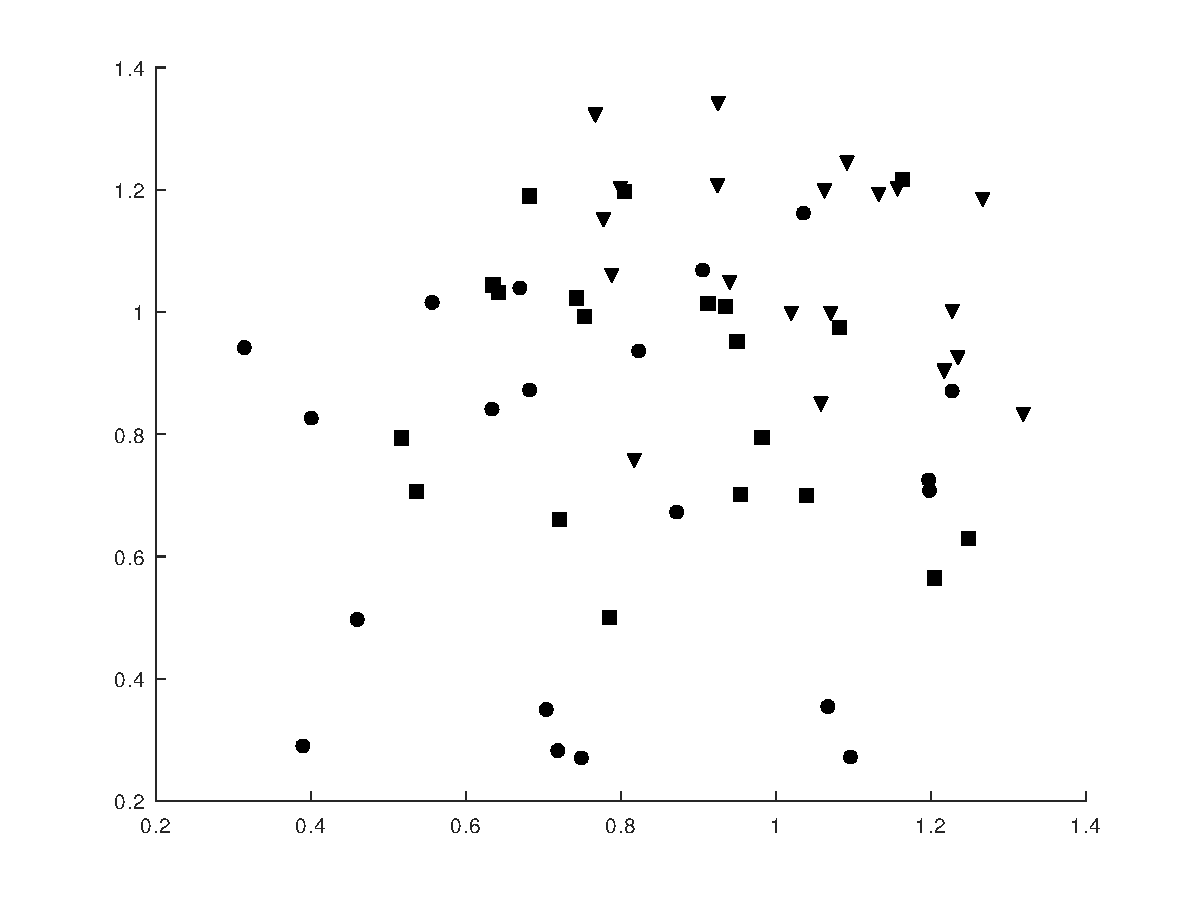
\includegraphics[width=0.7\textwidth,height=0.7\textheight,keepaspectratio]{figures/scatterplot1.pdf}
 \caption{Gráfico de espalhamento utilizando tipo de elemento para distinguir os grupos.}
 \label{fig-scatterplot1}
\end{figure}


\framebreak

\begin{figure}[h]
 \centering
  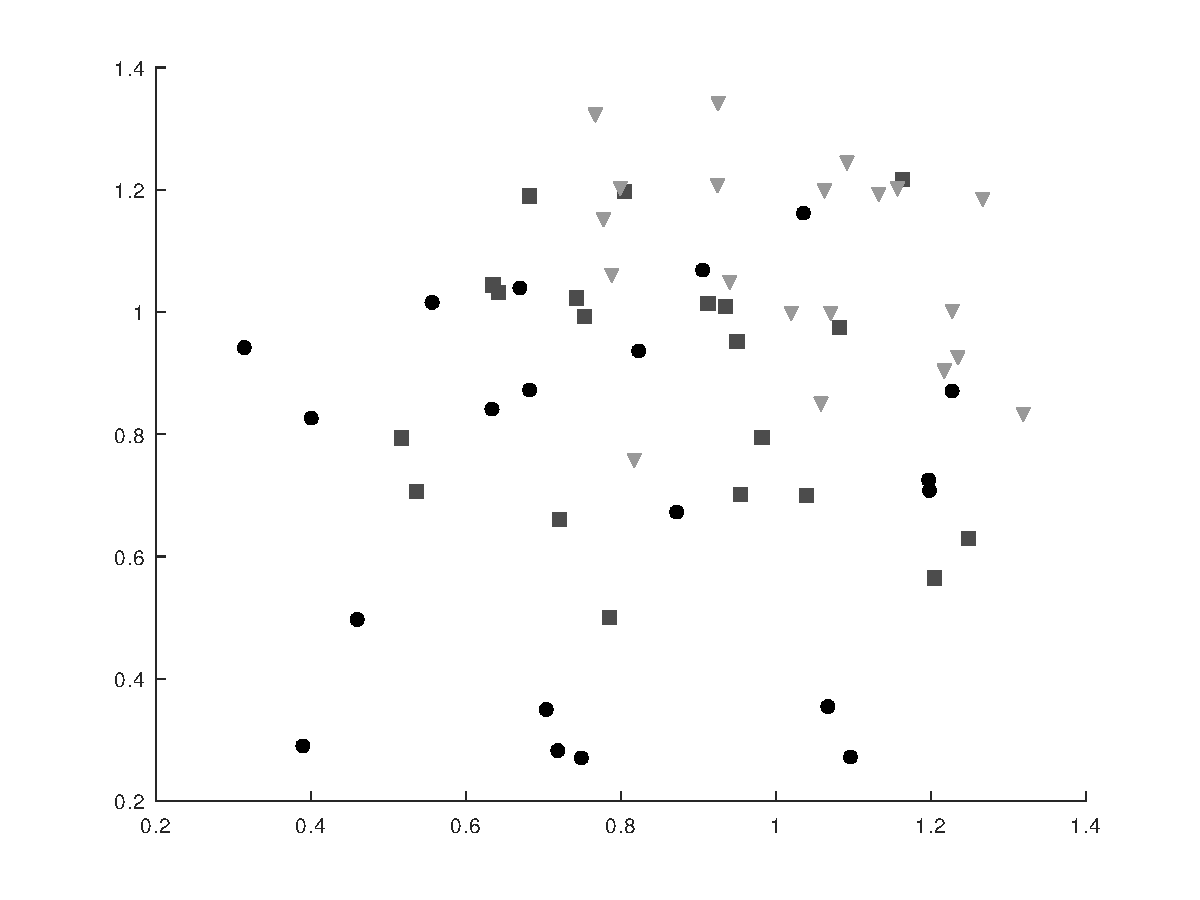
\includegraphics[width=0.7\textwidth,height=0.7\textheight,keepaspectratio]{figures/scatterplot2.pdf}
 \caption{Gráfico de espalhamento utilizando também a cor para distinguir os grupos.}
 \label{fig-scatterplot2}
\end{figure}

\end{frame}


\begin{frame}[allowframebreaks,fragile]
\frametitle{Limitações de alguns gráficos}
\begin{lstlisting}[language=Octave, label=lst-scatters, caption={Gráfico de espalhamento com 3 grupos.}, postbreak=\mbox{$\hookrightarrow$\space}, basicstyle=\fontsize{8}{10}\selectfont\ttfamily]
x = [4 11 22 29 38 42 49 7 13 22 31 39 42 49 7 14 23 32 40 43 55 9 15 27 33 40 45 58 10 15 27 33 40 47 66 10 20 28 35 40 48 72 11 21 28 38 42 48 73];
plot(x,0,'ko'); ylim ([-5 5]);
set(gca,'Visible','off')
axes('Position',get(gca,'Position'),'XAxisLocation','bottom','YAxisLocation','left', 'Color','none','XTickLabel',get(gca,'XTickLabel'),'YTickLabel',get(gca,'YTickLabel'),'XColor','k','YColor','k','LineWidth',1,'TickDir','out');
print -dsvg strip1.svg

plot(x,0.125*randn(1,length(x)),'ko'); ylim ([-5 5]);
set(gca,'Visible','off')
axes('Position',get(gca,'Position'),'XAxisLocation','bottom','YAxisLocation','left', 'Color','none','XTickLabel',get(gca,'XTickLabel'),'YTickLabel',get(gca,'YTickLabel'),'XColor','k','YColor','k','LineWidth',1,'TickDir','out');
print -dsvg strip2.svg
\end{lstlisting}

\framebreak

\begin{figure}[h]
 \centering
  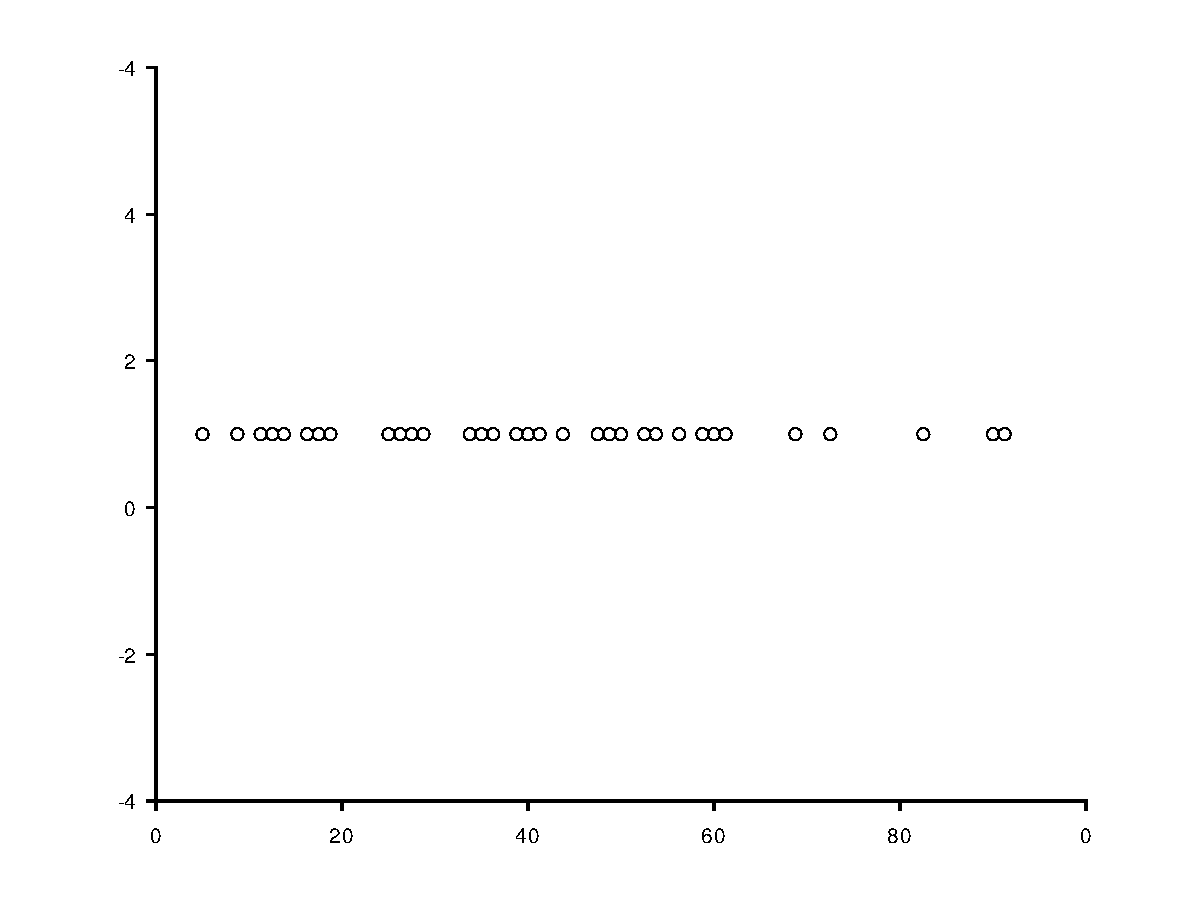
\includegraphics[width=0.7\textwidth,height=0.7\textheight,keepaspectratio]{figures/strip1.pdf}
 \caption{Strip plot.}
 \label{fig-strip1}
\end{figure}

\framebreak

\begin{figure}[h]
 \centering
  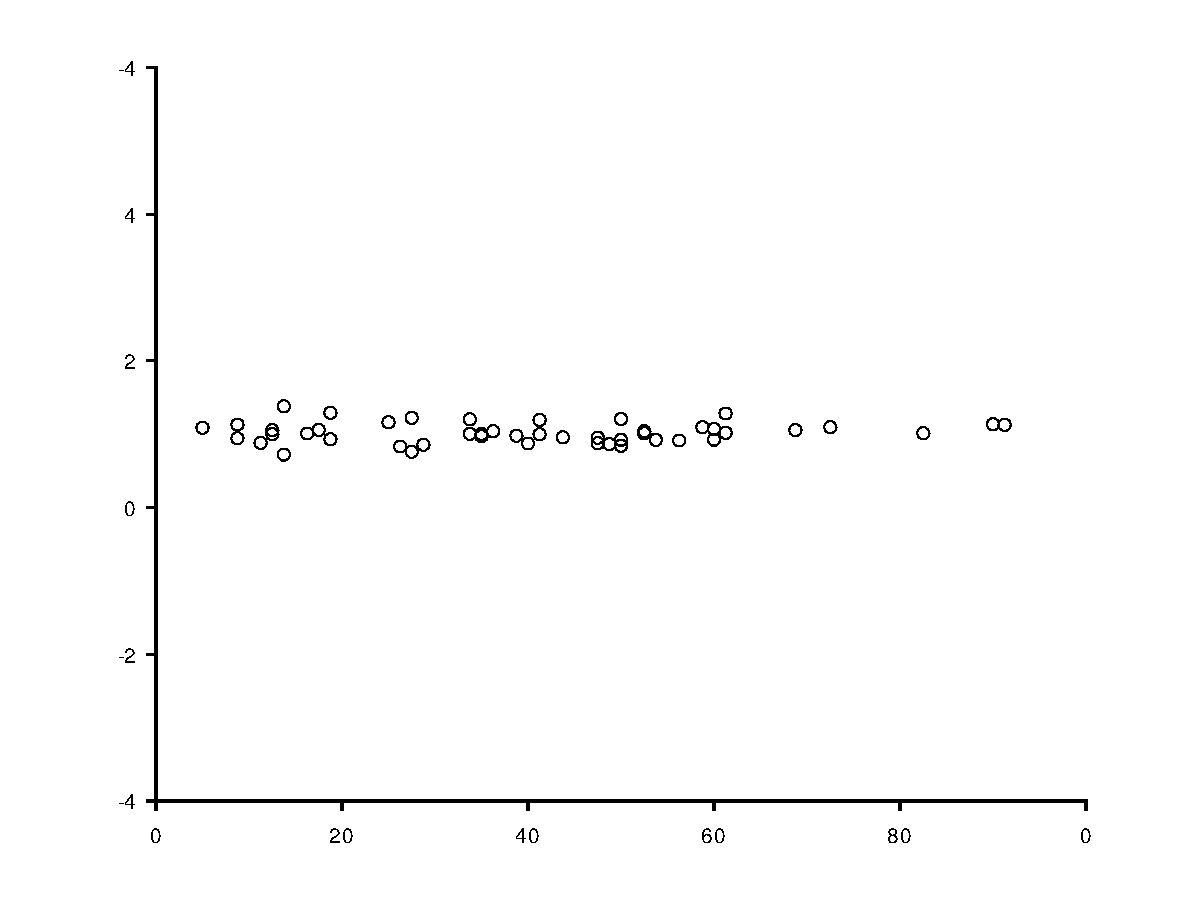
\includegraphics[width=0.7\textwidth,height=0.7\textheight,keepaspectratio]{figures/strip2.pdf}
 \caption{Strip plot com Jittering - possibilita a visualização de pontos sobrepostos.}
 \label{fig-strip2}
\end{figure}
\end{frame}


\begin{frame}
\frametitle{Razão de aspecto}

\begin{figure}[h]
 \centering
  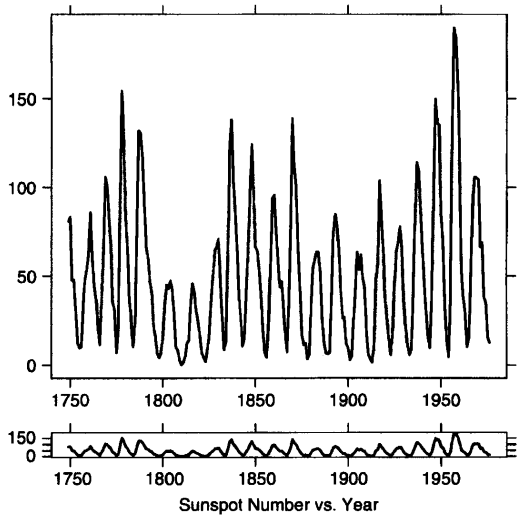
\includegraphics[width=0.5\textwidth,height=0.7\textheight,keepaspectratio]{figures/sunspots.png}
 \caption{Número de manchas solares ao longo dos anos \cite{robbins_creating_2013}. Razão de aspecto 0.8 (gráfico de cima) e 0.055 (gráfico de baixo).}
 \label{fig-sunspots}
\end{figure}

\end{frame}
\note{
Note como a razão de aspecto influencia na percepção dos altos e baixos no gráfico.
No gráfico de baixo fica evidente a diferença na velocidade de subida e descida.
}


\begin{frame}
\frametitle{Razão de aspecto e referência zero}
\begin{figure}[h]
 \centering
  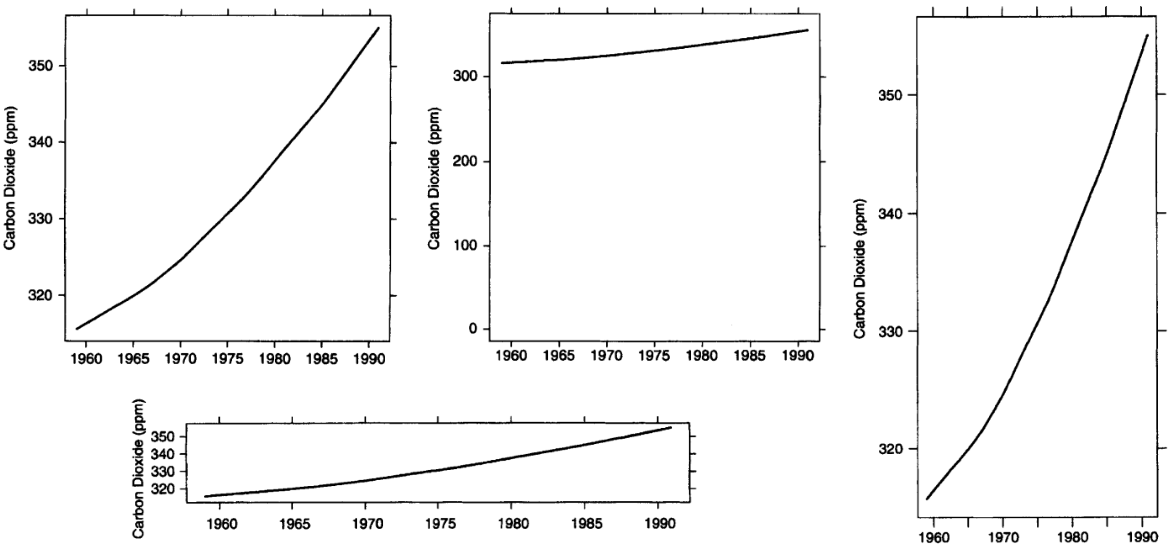
\includegraphics[width=0.8\textwidth,height=0.7\textheight,keepaspectratio]{figures/carbondioxide.png}
 \caption{Nível de dióxido de carbono na atmosfera \cite{robbins_creating_2013}.}
 \label{fig-carbondioxide}
\end{figure}
\end{frame}


\begin{frame}
\frametitle{Escala logarítmica}
\begin{figure}[h]
 \centering
  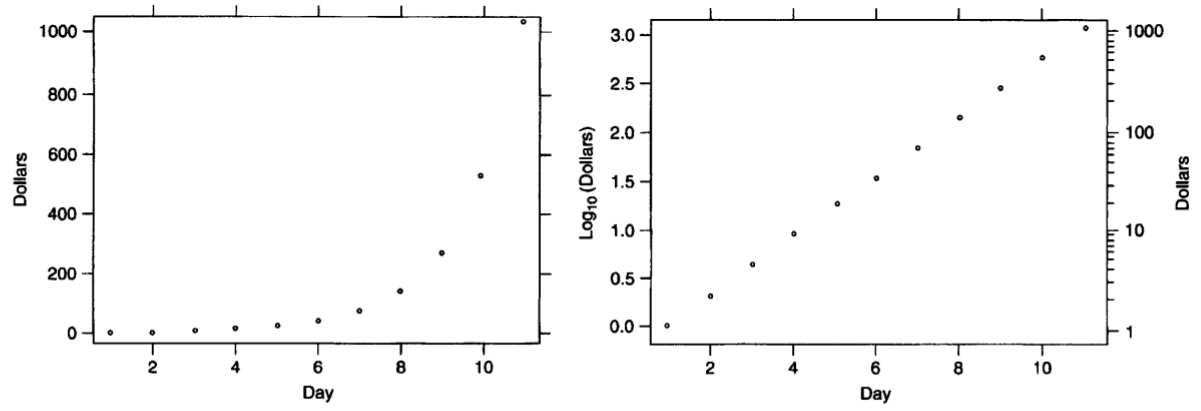
\includegraphics[width=0.8\textwidth,height=0.7\textheight,keepaspectratio]{figures/uselogscale.png}
 \caption{Uso da escala logarítmica \cite{robbins_creating_2013}. Os valores dobram a cada dia.}
 \label{fig-uselogscale}
\end{figure}
\end{frame}


\begin{frame}
\frametitle{Eixo y duplo}
\begin{figure}[h]
 \centering
  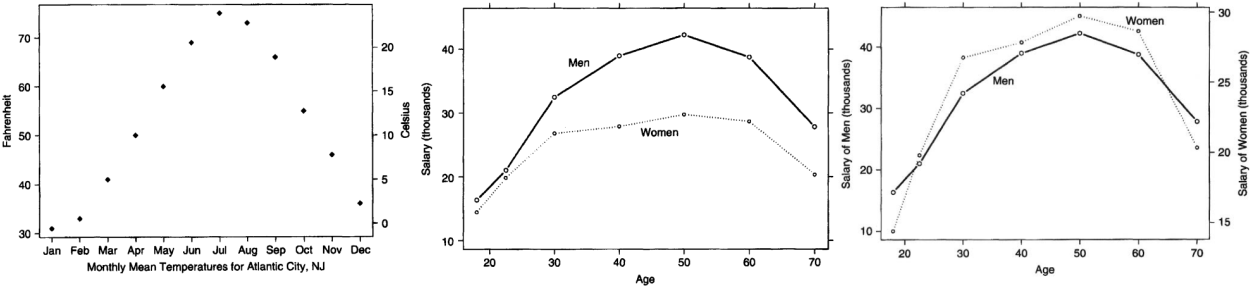
\includegraphics[width=\textwidth,height=0.7\textheight,keepaspectratio]{figures/dyaxis.png}
 \caption{Uso de eixo y duplo \cite{robbins_creating_2013}.}
 \label{fig-dyaxis}
\end{figure}
Evite usar eixo y duplo. Note como uma má escolha pode levar a uma interpretação errônea.
\end{frame}

\begin{frame}
\frametitle{Variáveis com extensões diferentes}
\begin{figure}[h]
 \centering
  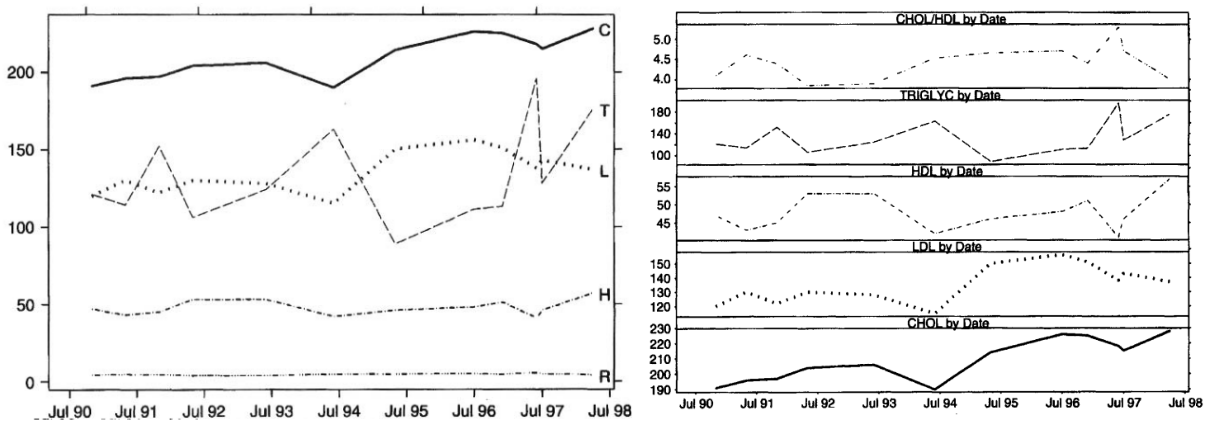
\includegraphics[width=0.9\textwidth,height=0.7\textheight,keepaspectratio]{figures/range.png}
 \caption{Nível sanguíneo \cite{robbins_creating_2013}.}
 \label{fig-range}
\end{figure}
\end{frame}

\begin{frame}
\frametitle{Máxima, mínima e média ao longo do tempo}
\begin{figure}[h]
 \centering
  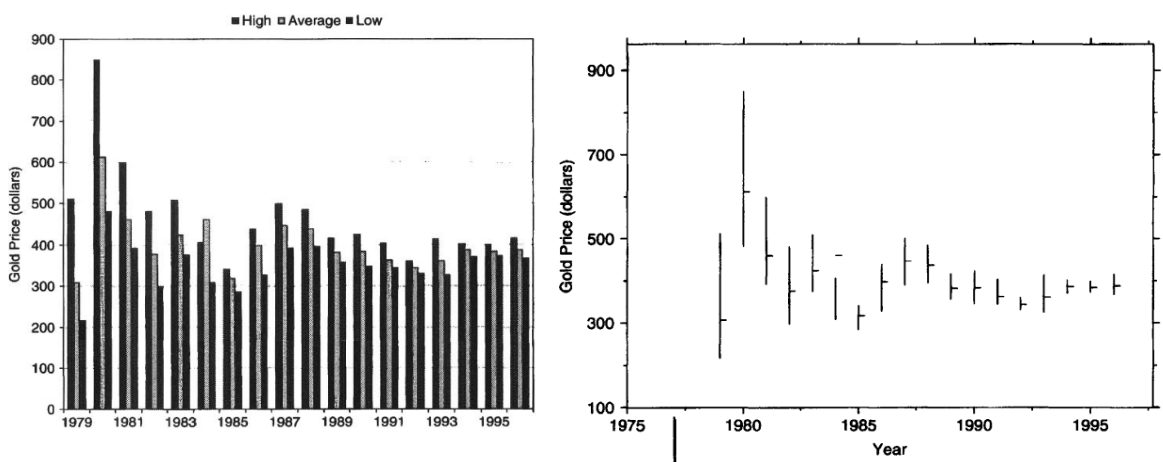
\includegraphics[width=0.9\textwidth,height=0.7\textheight,keepaspectratio]{figures/maxminmeanchart.png}
 \caption{Preço do ouro \cite{robbins_creating_2013}.}
 \label{fig-maxminmeanchart}
\end{figure}
\end{frame}

\begin{frame}[allowframebreaks]
\frametitle{Agregando, simplificando e ordenando}
\begin{figure}[h]
 \centering
  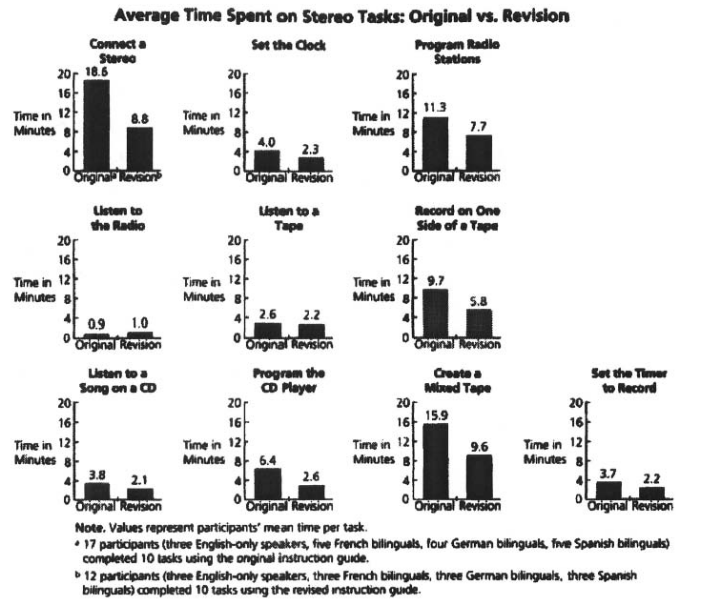
\includegraphics[width=0.9\textwidth,height=0.7\textheight,keepaspectratio]{figures/vcrmanual01.png}
 \caption{Tempo gasto para ler uma secção do manual e executar a tarefa \cite{robbins_creating_2013}.}
 \label{fig-vcrmanual01}
\end{figure}

\framebreak

\begin{figure}[h]
 \centering
  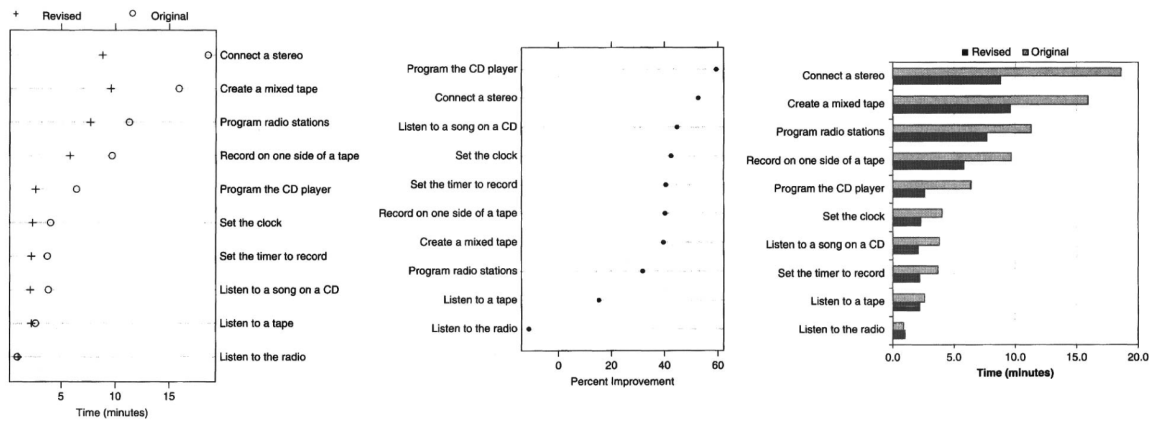
\includegraphics[width=\textwidth,height=0.7\textheight,keepaspectratio]{figures/vcrmanual02.png}
 \caption{Tempo gasto para ler uma secção do manual e executar a tarefa \cite{robbins_creating_2013}.}
 \label{fig-vcrmanual02}
\end{figure}
\end{frame}


\begin{frame}[allowframebreaks,fragile]
\frametitle{Dados de crescimento de dentes}
Vamos analisar os dados de crescimento de dente em Porquinho-da-Índia disponíveis no R (\emph{Tooth Growth Data}).
Os dados mostram o crescimento de odontoblasto\footnote{Odontoblasto é um tipo de células colunares responsáveis pela síntese de matriz da pré-dentina.}
em 10 porquinhos-da-índia a 3 dosagens de vitamina C (0.5, 1, e 2 mg) com dois métodos de entrega (suco de laranja (OJ) e ácido ascórbico (VC)).
Os dados apresentam 60 observações de 3 variáveis (tamanho do dente, tipo de suplemento e dosagem).

\vspace{3ex}
\fullcite{crampton_growth_1947}

\begin{lstlisting}[language=R, label=lst-tooth-0, caption={Resumo dos dados.}, postbreak=\mbox{$\hookrightarrow$\space}, basicstyle=\fontsize{8}{10}\selectfont\ttfamily]
> data(ToothGrowth)
> summary(ToothGrowth)
      len        supp         dose      
 Min.   : 4.20   OJ:30   Min.   :0.500  
 1st Qu.:13.07   VC:30   1st Qu.:0.500  
 Median :19.25           Median :1.000  
 Mean   :18.81           Mean   :1.167  
 3rd Qu.:25.27           3rd Qu.:2.000  
 Max.   :33.90           Max.   :2.000  
\end{lstlisting}

\begin{lstlisting}[language=R, label=lst-tooth-1, caption={Gráfico de pontos evidenciando cada amostra.}, postbreak=\mbox{$\hookrightarrow$\space}, basicstyle=\fontsize{8}{10}\selectfont\ttfamily]
> library(ggplot2)
> library(dplyr)
> ggplot(ToothGrowth, aes(x= dose, y= len)) + geom_point(aes(color=supp)) + theme_minimal()
> ggsave('tooth01.pdf')
\end{lstlisting}

\begin{figure}[h]
 \centering
  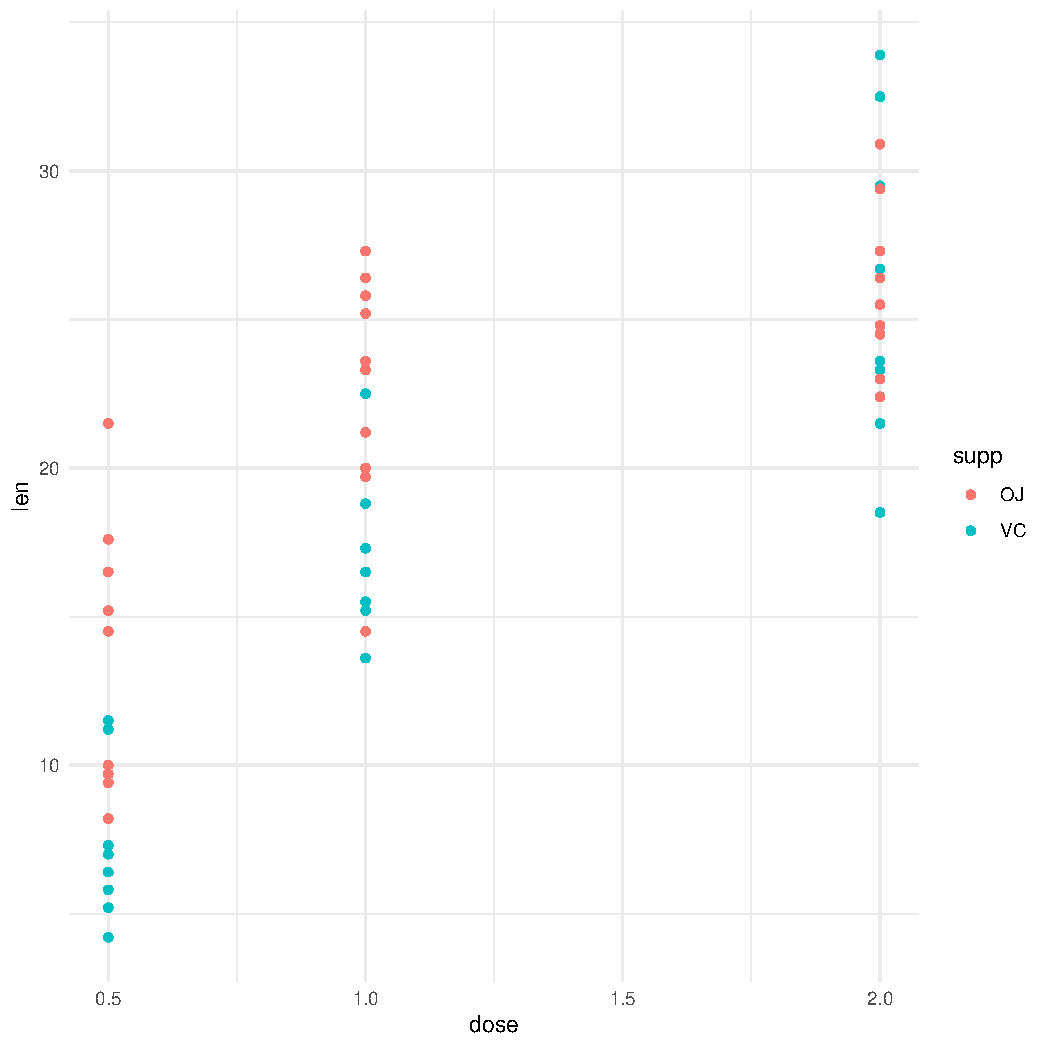
\includegraphics[width=0.7\textwidth,height=0.7\textheight,keepaspectratio]{figures/tooth01.pdf}
 \caption{Gráfico de pontos evidenciando as amostras. Gerado pelo código na lista \ref{lst-tooth-1}.}
 \label{fig-tooth01}
\end{figure}

\begin{lstlisting}[language=R, label=lst-tooth-2, caption={Sumário dos dados.}, postbreak=\mbox{$\hookrightarrow$\space}, basicstyle=\fontsize{8}{10}\selectfont\ttfamily]
> ToothGrowth %>% group_by(supp,dose) %>% summarize(lenmean=mean(len), lensd=sd(len), count = n())
`summarise()` has grouped output by 'supp'. You can override using the `.groups` argument.
# A tibble: 6 x 5
# Groups:   supp [2]
  supp   dose lenmean lensd count
  <fct> <dbl>   <dbl> <dbl> <int>
1 OJ      0.5   13.2   4.46    10
2 OJ      1     22.7   3.91    10
3 OJ      2     26.1   2.66    10
4 VC      0.5    7.98  2.75    10
5 VC      1     16.8   2.52    10
6 VC      2     26.1   4.80    10
\end{lstlisting}

\framebreak

\begin{lstlisting}[language=R, label=lst-tooth-jitter, caption={Jitter.}, postbreak=\mbox{$\hookrightarrow$\space}, basicstyle=\fontsize{8}{10}\selectfont\ttfamily]
ggplot(ToothGrowth, aes(x= dose, y= len)) + geom_jitter(aes(color=supp), shape=16, position=position_jitter(0.1)) + theme_minimal()
ggsave('tooth-jitter.pdf')
\end{lstlisting}

\begin{figure}[h]
 \centering
  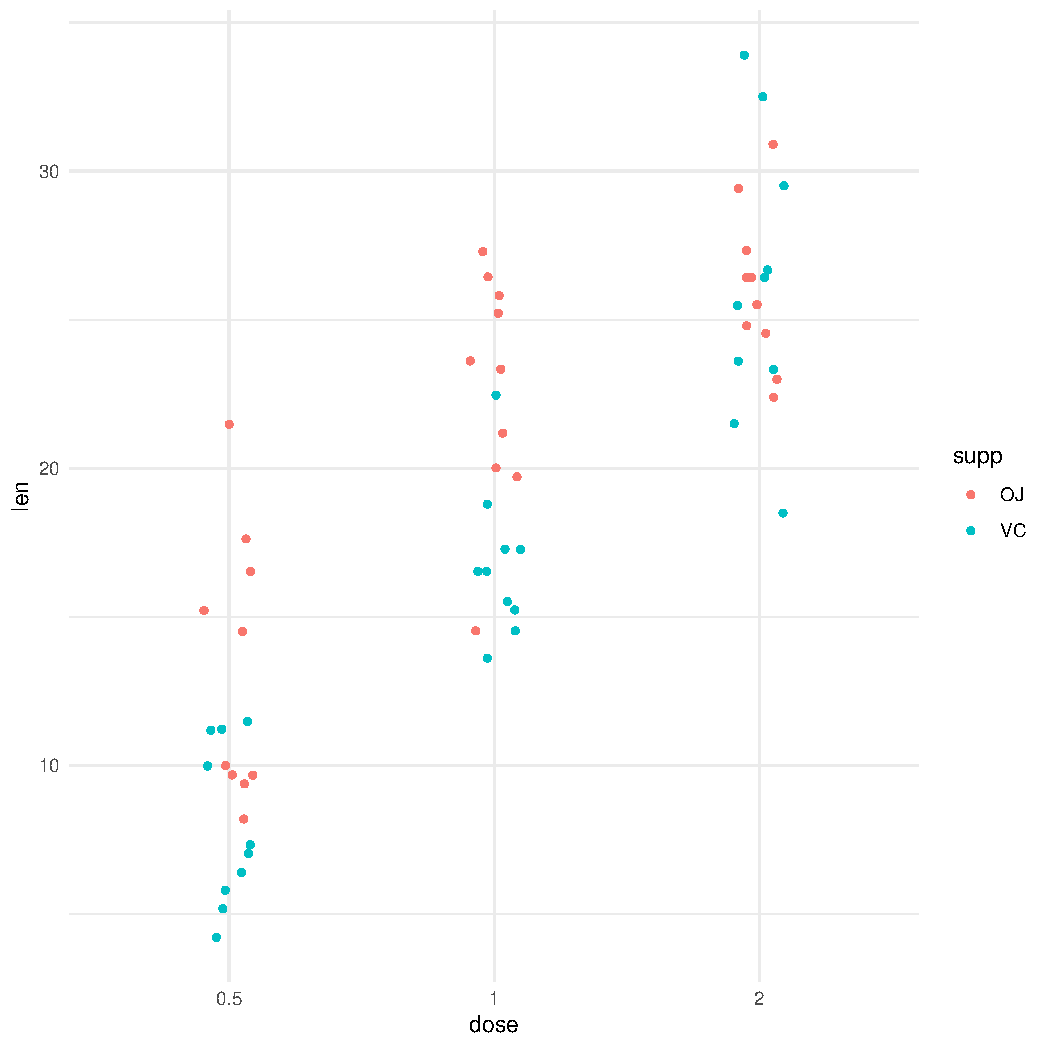
\includegraphics[width=0.7\textwidth,height=0.7\textheight,keepaspectratio]{figures/tooth-jitter.pdf}
 \caption{Gráfico de \emph{jitter} evidenciando as amostras. Gerado pelo código na lista \ref{lst-tooth-jitter}.}
 \label{fig-tooth-jitter}
\end{figure}


\framebreak

\begin{lstlisting}[language=R, label=lst-tooth-3, caption={Box plot.}, postbreak=\mbox{$\hookrightarrow$\space}, basicstyle=\fontsize{8}{10}\selectfont\ttfamily]
library(ggplot2)
ToothGrowth$dose <- as.factor(ToothGrowth$dose)
ggplot(ToothGrowth, aes(x=dose, y=len)) + geom_boxplot() + theme_minimal()
ggsave('tooth02.pdf')
\end{lstlisting}

\begin{figure}[h]
 \centering
  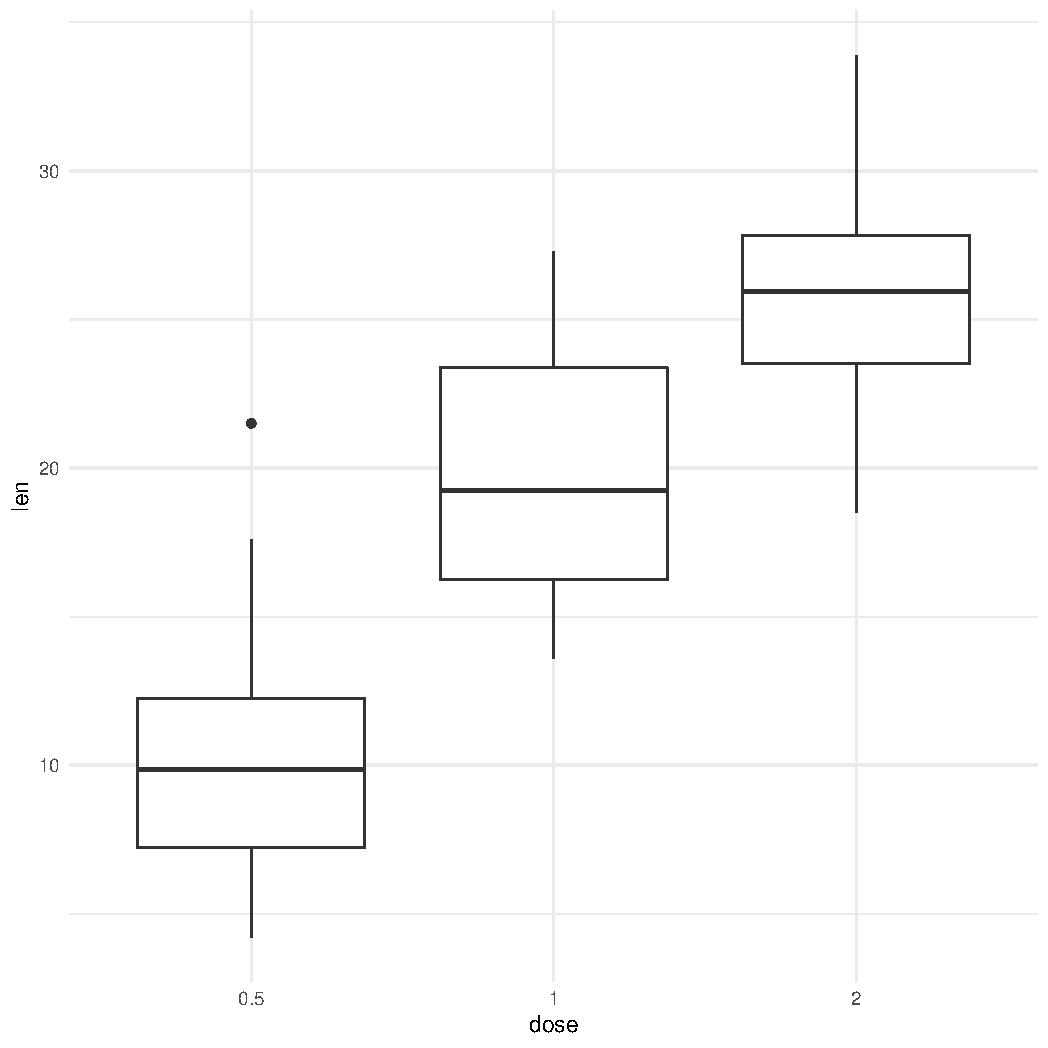
\includegraphics[width=0.7\textwidth,height=0.7\textheight,keepaspectratio]{figures/tooth02.pdf}
 \caption{Diagrama de caixa (\emph{Box plot}). Gerado pelo código na lista \ref{lst-tooth-3}.}
 \label{fig-tooth02}
\end{figure}

\framebreak

\begin{lstlisting}[language=R, label=lst-tooth-4, caption={Box plot.}, postbreak=\mbox{$\hookrightarrow$\space}, basicstyle=\fontsize{8}{10}\selectfont\ttfamily]
ggplot(ToothGrowth, aes(x=dose, y=len)) + geom_boxplot(notch=TRUE, outlier.colour="red", outlier.shape=8, outlier.size=4) + coord_flip() + theme_minimal()
ggsave('tooth03.pdf')
\end{lstlisting}

\begin{figure}[h]
 \centering
  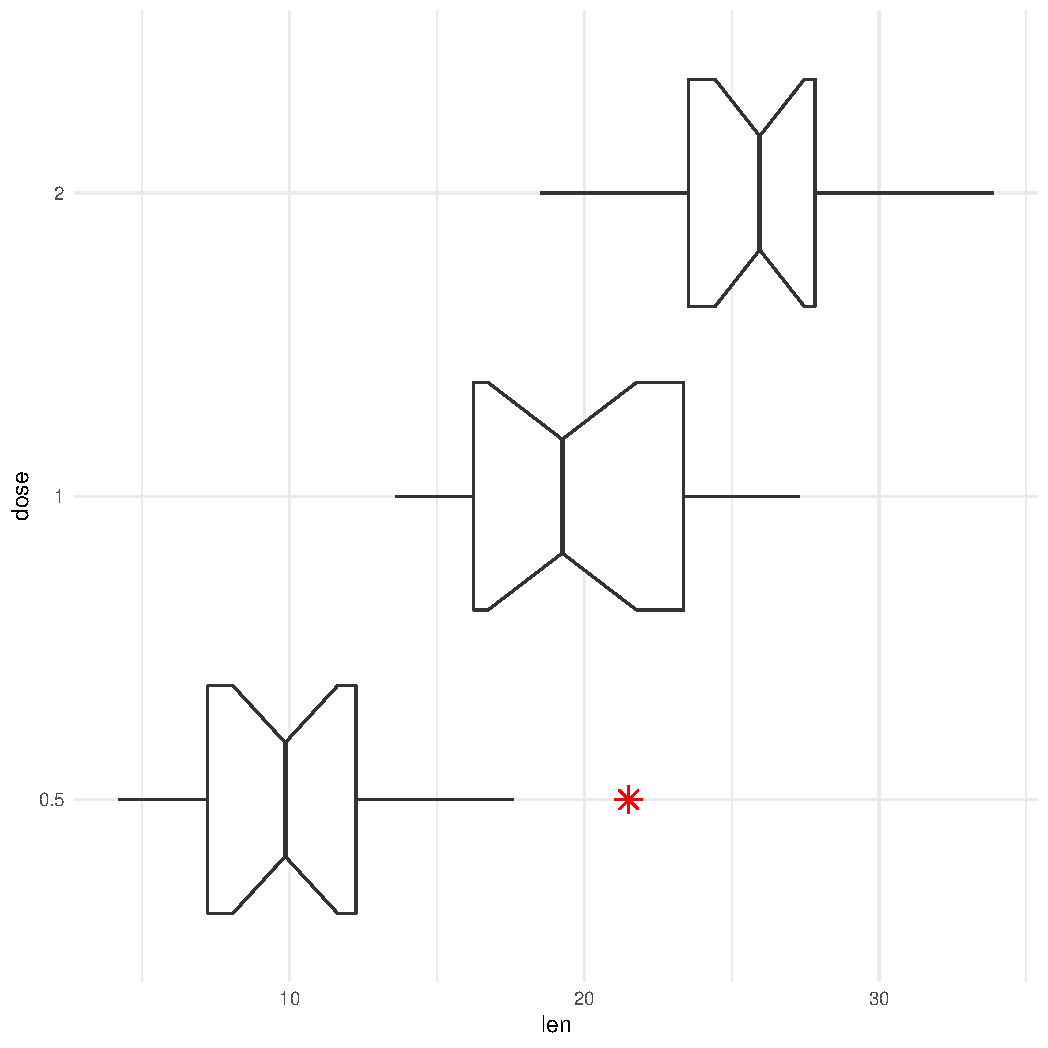
\includegraphics[width=0.7\textwidth,height=0.7\textheight,keepaspectratio]{figures/tooth03.pdf}
 \caption{Diagrama de caixa (\emph{Box plot}). Gerado pelo código na lista \ref{lst-tooth-4}.}
 \label{fig-tooth03}
\end{figure}

\framebreak

\begin{lstlisting}[language=R, label=lst-tooth-5, caption={Box plot.}, postbreak=\mbox{$\hookrightarrow$\space}, basicstyle=\fontsize{8}{10}\selectfont\ttfamily]
ggplot(ToothGrowth, aes(x=dose, y=len, fill=dose)) + geom_boxplot(notch=TRUE, outlier.colour="red", outlier.size=2) + coord_flip() + theme_minimal() + theme(legend.position="bottom")
ggsave('tooth04.pdf')
\end{lstlisting}

\begin{figure}[h]
 \centering
  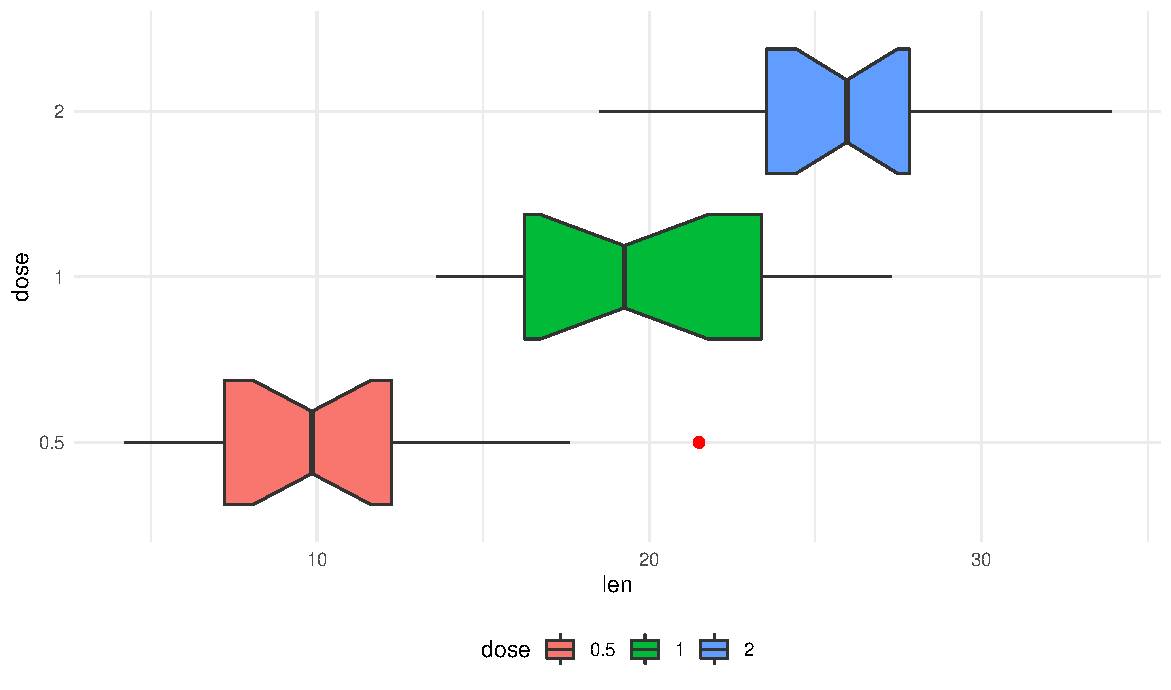
\includegraphics[width=0.7\textwidth,height=0.7\textheight,keepaspectratio]{figures/tooth04.pdf}
 \caption{Diagrama de caixa (\emph{Box plot}). Gerado pelo código na lista \ref{lst-tooth-5}.}
 \label{fig-tooth04}
\end{figure}

\framebreak

\begin{lstlisting}[language=R, label=lst-tooth-6, caption={Box plot.}, postbreak=\mbox{$\hookrightarrow$\space}, basicstyle=\fontsize{8}{10}\selectfont\ttfamily]
ggplot(ToothGrowth, aes(x=dose, y=len, fill=supp)) + geom_boxplot() + theme_minimal()
ggsave('/tmp/tooth05.pdf')
\end{lstlisting}

\begin{figure}[h]
 \centering
  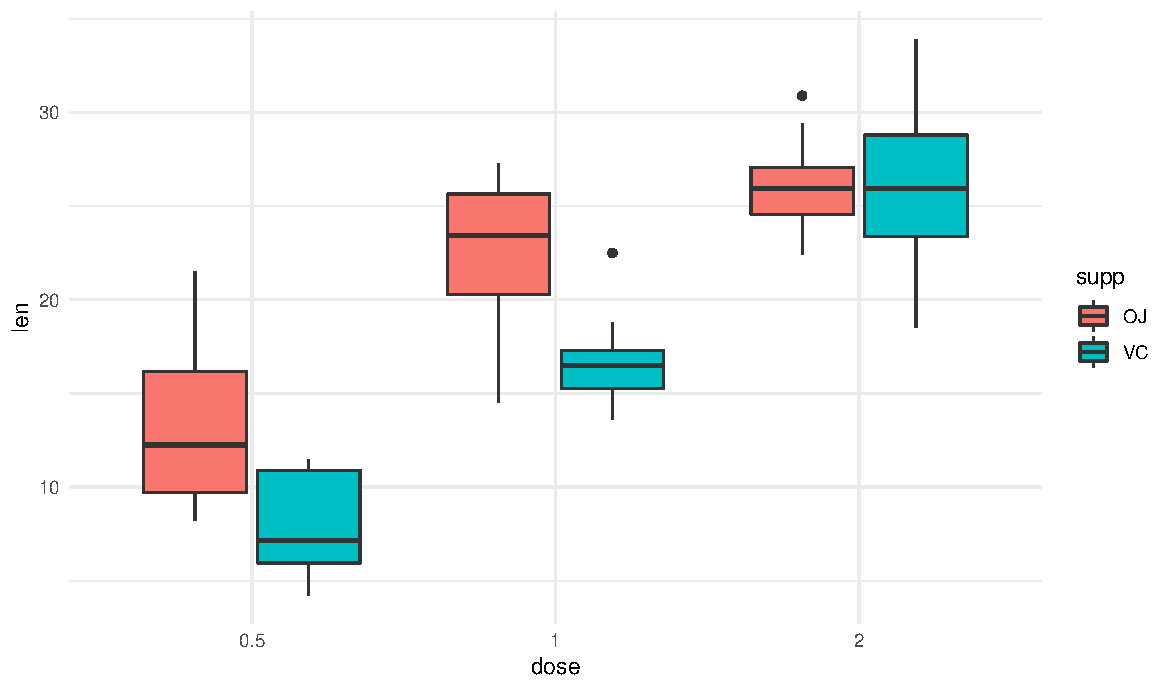
\includegraphics[width=0.7\textwidth,height=0.7\textheight,keepaspectratio]{figures/tooth05.pdf}
 \caption{Diagrama de caixa (\emph{Box plot}). Gerado pelo código na lista \ref{lst-tooth-6}.}
 \label{fig-tooth05}
\end{figure}

\framebreak

\begin{footnotesize}
Examining Tooth Growth Data in R\\
\url{https://rpubs.com/garedwards/107023}

\begin{quote}
Conclusions and Assumptions

Based off this data we can conclude the following:
\begin{itemize}
\item As dosage increases, tooth length increases regardless of supplement method.
\item At the 0.5 mg and 1.0 mg dosage the OJ supplement method leads to more tooth growth than the VC method.
\item At the 2.0 mg dosage, there is no significant difference between the OJ and VC supplement methods.
\end{itemize}

Assumptions
\begin{itemize}
\item We assume that the measurements are not paired.
\item We do not assume that the variances are equal (var.equal=FALSE)
\item We assume the populations are independent, that there was no crossover between the subjects and dosage.
\item We assume that the guinea pigs were truly selected at random so no conflating factors influence the results.
\end{itemize}
\end{quote}
\end{footnotesize}
\end{frame}


\begin{frame}[allowframebreaks]
\frametitle{box plot explained}

\begin{figure}[h]
 \centering
  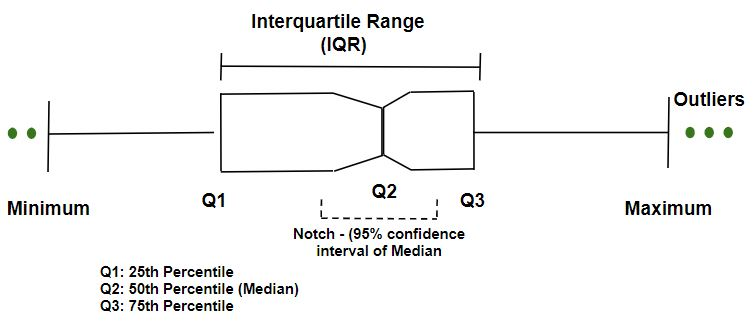
\includegraphics[width=0.8\textwidth,height=0.6\textheight,keepaspectratio]{figures/fake-data-notch-boxplot.jpg}
 \caption{Explicando o diagrama de caixa (\emph{box plot}). Fonte: \url{https://www.geeksforgeeks.org/understanding-different-box-plot-with-visualization/}.}
 \label{fig-boxplot-explained}
\end{figure}

\framebreak

\begin{figure}[h]
 \centering
  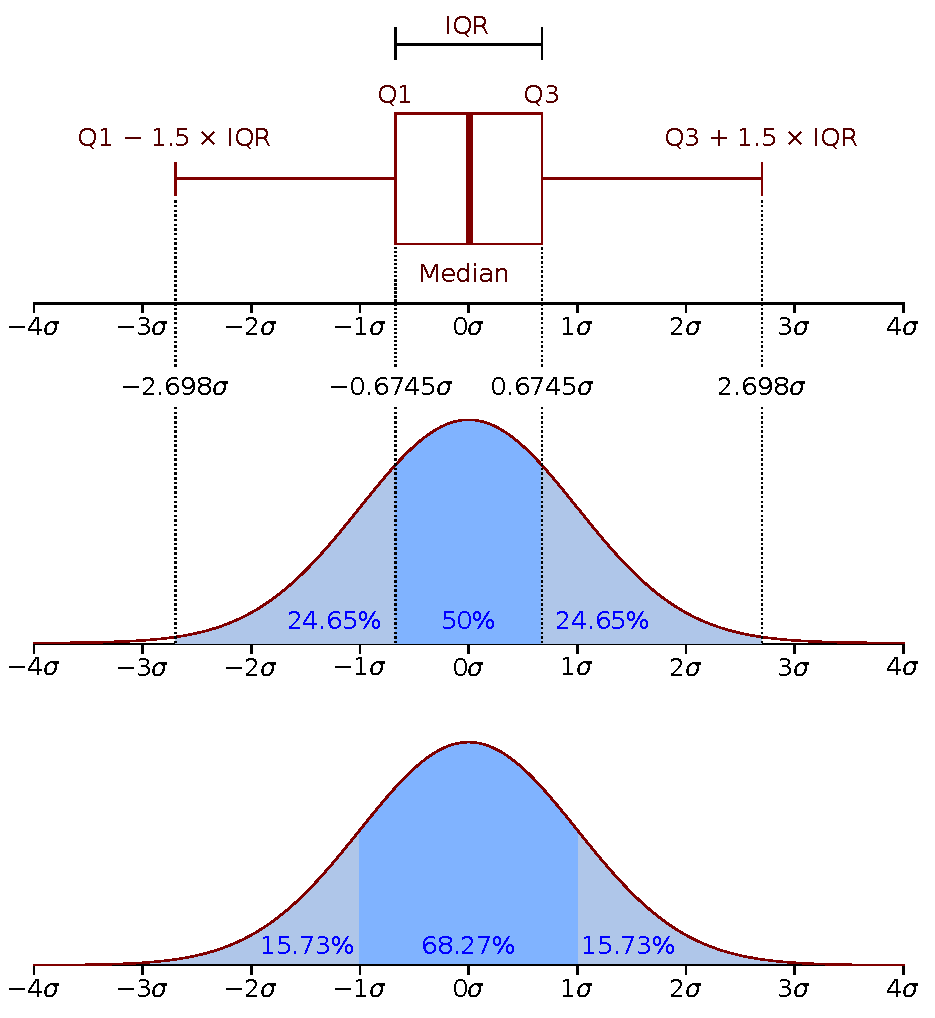
\includegraphics[width=0.5\textwidth,height=0.72\textheight,keepaspectratio]{figures/Boxplot_vs_PDF.pdf}
 \caption{Box plot e distribuição normal (Wikipedia).}
 \label{fig-boxplot-normal}
\end{figure}


\end{frame}



\begin{frame}[allowframebreaks,fragile]
\frametitle{}
\begin{lstlisting}[language=R, label=lst-nycflights13-A, caption={Box plot.}, postbreak=\mbox{$\hookrightarrow$\space}, basicstyle=\fontsize{8}{10}\selectfont\ttfamily]
library(nycflights13)
tempdata <- aggregate(temp ~ month + day, data=weather, mean)
pdf('nycflights13-A.pdf')
with(tempdata, monthplot(temp, times=day , phase=month, ylab = "temp"))
dev.off()
\end{lstlisting}

\begin{figure}[h]
 \centering
  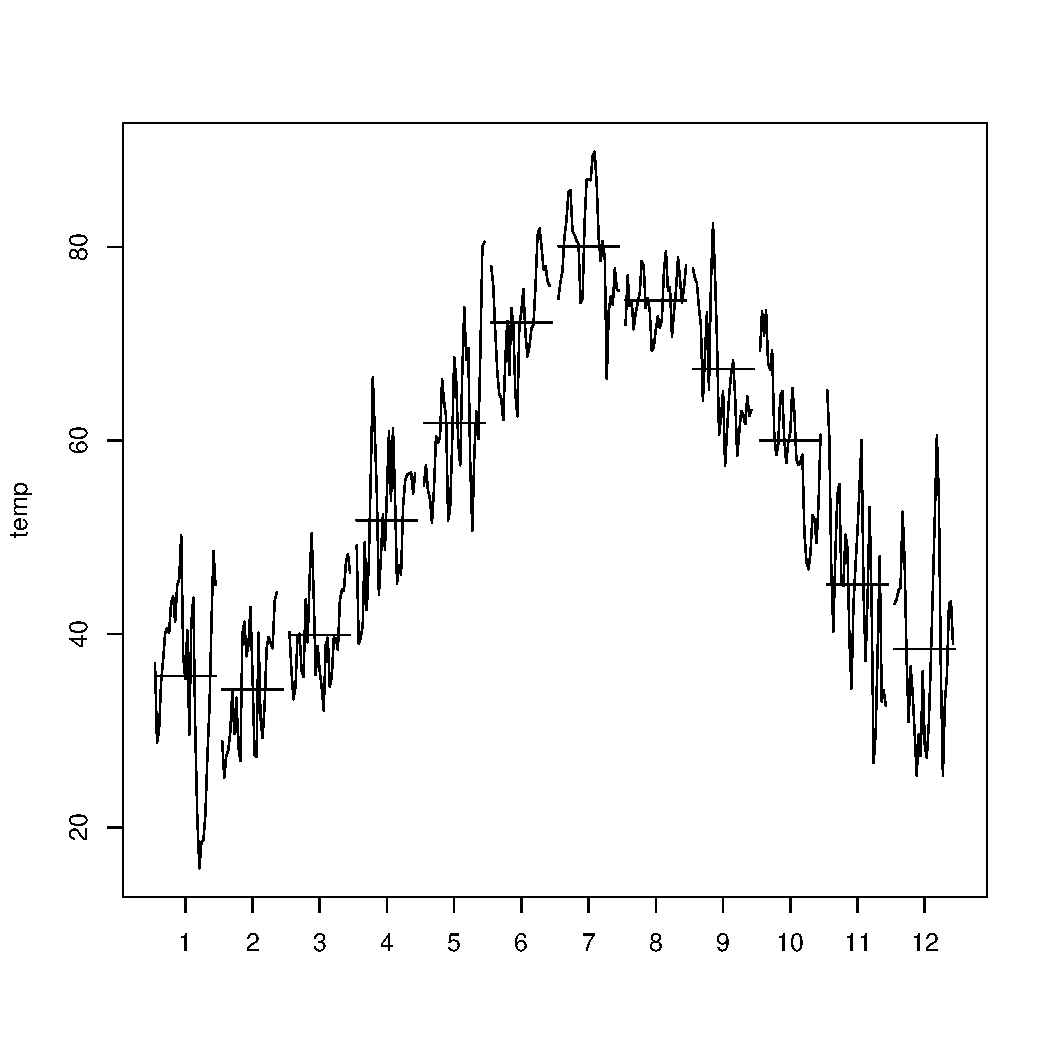
\includegraphics[width=0.7\textwidth,height=0.7\textheight,keepaspectratio]{figures/nycflights13-A.pdf}
 \caption{Temperatura em NYC ao longo de 2013. Base de dados \texttt{nycflights13}. Gerado pelo código na lista \ref{lst-nycflights13-A}.}
 \label{fig-nycflights13-A}
\end{figure}

\framebreak

\begin{lstlisting}[language=R, label=lst-nycflights13-B, caption={Box plot.}, postbreak=\mbox{$\hookrightarrow$\space}, basicstyle=\fontsize{8}{10}\selectfont\ttfamily]
library('ggplot2')
months.labs <- c("Jan","Feb","Mar","Apr","May","Jun","Jul","Aug","Sep","Oct","Nov","Dez")
names(months.labs) <- c(1,2,3,4,5,6,7,8,9,10,11,12)
ggplot(tempdata, aes(x=month+day, y=temp)) + geom_line() + stat_smooth(method="lm", formula=y~1, se=F) + facet_wrap(~month, nrow=1, labeller = labeller(month=months.labs)) + theme_minimal() + theme(axis.text.x = element_blank(), axis.title.x = element_blank(), panel.grid.major = element_blank(), panel.grid.minor = element_blank()) + labs(title="Temperature in NYC in 2013", y="Temperature (°F)")
ggsave('nycflights13-B.pdf')
\end{lstlisting}

\begin{figure}[h]
 \centering
  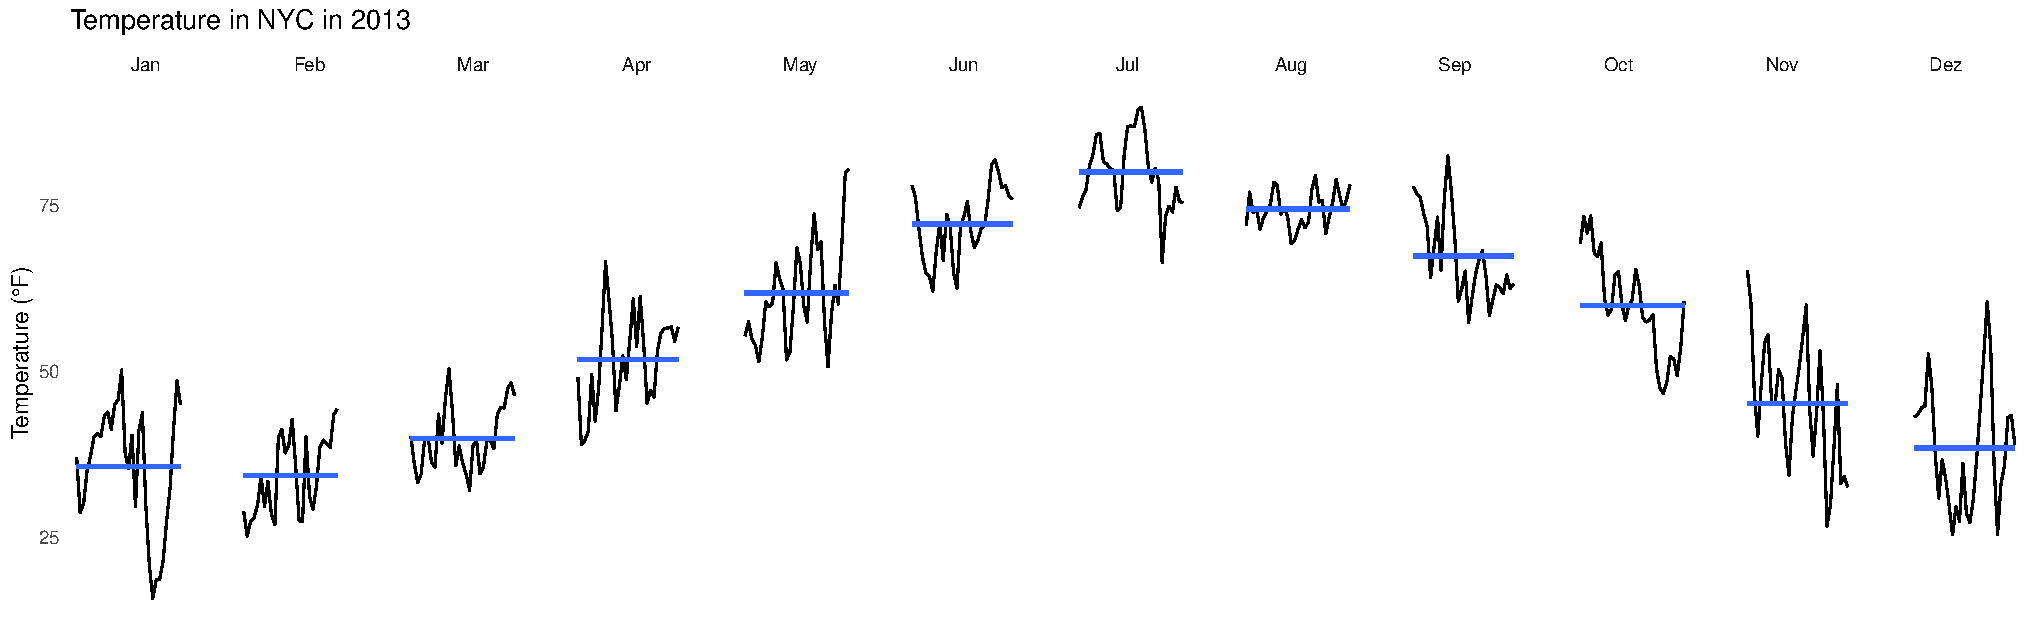
\includegraphics[width=\textwidth,height=0.7\textheight,keepaspectratio]{figures/nycflights13-B.pdf}
 \caption{Temperatura em NYC ao longo de 2013. Base de dados \texttt{nycflights13}. Gerado pelo código na lista \ref{lst-nycflights13-B}.}
 \label{fig-nycflights13-B}
\end{figure}

\url{https://cran.r-project.org/web/packages/nycflights13/index.html}

\end{frame}


\begin{frame}[allowframebreaks,fragile]
\frametitle{Pizza e Waffle}

\begin{lstlisting}[language=R, label=lst-irisspecies-pie, caption={Gráfico pizza.}, postbreak=\mbox{$\hookrightarrow$\space}, basicstyle=\fontsize{8}{10}\selectfont\ttfamily]
library(ggplot2)
ggplot(iris, aes(x="", fill=Species)) + geom_bar(width = 1) + coord_polar("y") + theme_minimal()
ggsave('irisspecies-pie.pdf')
\end{lstlisting}

\framebreak

\begin{figure}[h]
 \centering
 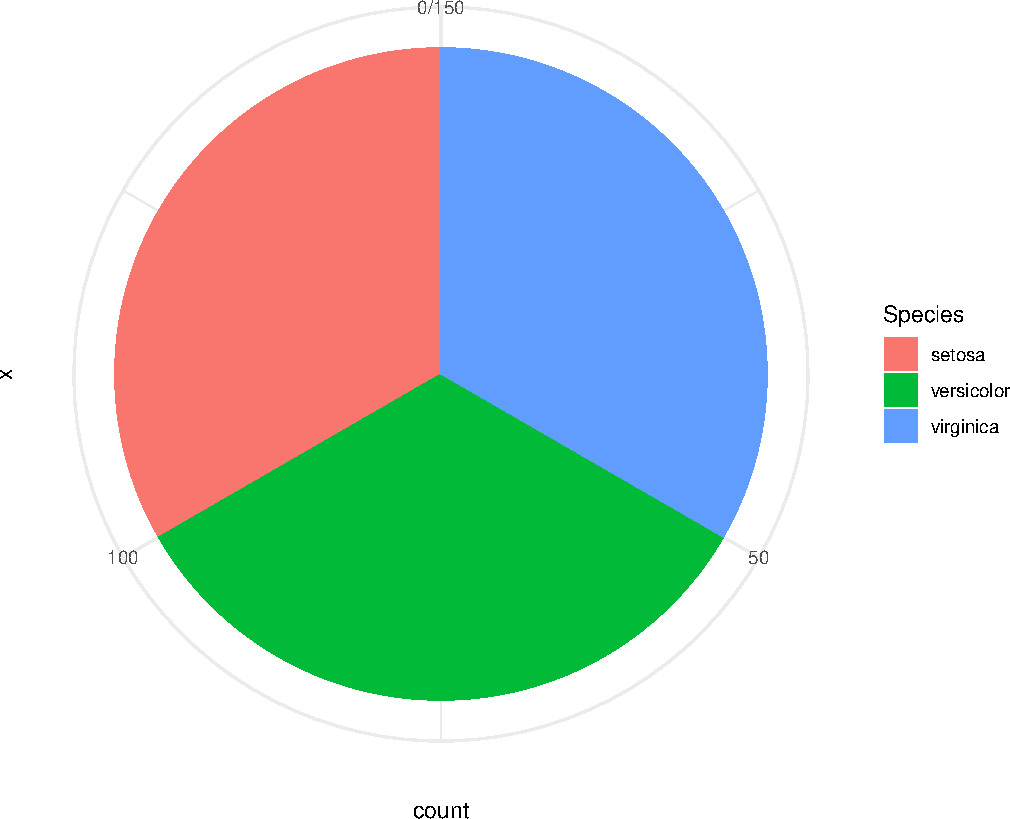
\includegraphics[width=0.7\textwidth,height=0.7\textheight,keepaspectratio]{figures/irisspecies-pie.pdf}
 \caption{Espécies da planta Iris.}
 \label{fig-irisspecies-pie}
\end{figure}

\framebreak

\begin{lstlisting}[language=R, label=lst-irisspecies-waffle, caption={Gráfico Waffle.}, postbreak=\mbox{$\hookrightarrow$\space}, basicstyle=\fontsize{8}{10}\selectfont\ttfamily]
library(ggwaffle)
iris$Species <- as.character(iris$Species)
waffle_data <- waffle_iron(iris, aes_d(group = Species))

ggplot(waffle_data, aes(x, y, fill = group)) + geom_waffle() + coord_equal() + scale_fill_waffle() + theme_waffle()
ggsave('irisspecies-waffle.pdf')
\end{lstlisting}

\framebreak

\begin{figure}[h]
 \centering
 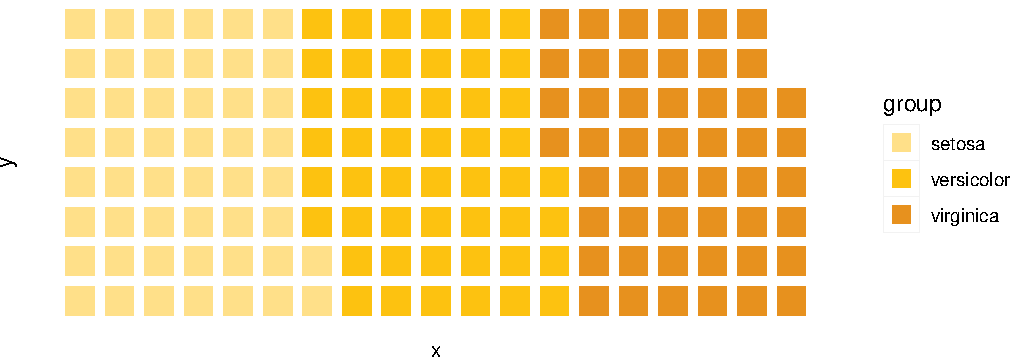
\includegraphics[width=0.9\textwidth,height=0.7\textheight,keepaspectratio]{figures/irisspecies-waffle.pdf}
 \caption{Espécies da planta Iris.}
 \label{fig-irisspecies-waffle}
\end{figure}

\end{frame}




\begin{frame}[allowframebreaks]
\frametitle{Percepção de elementos gráficos}
\begin{itemize}
\item ângulo  
\item área e volume 
\item matiz de cor
\item saturação de cor
\item densidade
\item comprimento
\item posição em uma escala
\item posição ao longo de escalas não alinhadas
\item inclinação
\end{itemize}

\begin{quote}
Distance and detection also play a role in our ability to decode
information from graphs. The closer together objects are, the
easier it is to judge attributes that compare them. As distance
between objects increases, accuracy of judgment decreases. It
is certainly easier to judge the difference in lengths of two bars
if they are next to one another than if they are pages apart.
\cite{robbins_creating_2013}
\end{quote}

\end{frame}



\begin{frame}
Sugestões de leitura: 
\vspace{2ex}

\fullcite{harford_florence}
\vspace{2ex}

\fullcite{tufte_visual_1999}
\vspace{2ex}

\fullcite{tufte_beautiful_2006}
\vspace{2ex}

\fullcite{knaflic_storytelling_2015}
\vspace{2ex}

\fullcite{robbins_creating_2013}
\end{frame}


\begin{frame}
\frametitle{Figuras}
Tipos de figuras:
\begin{itemize}
\item vetoriais (.pdf, .eps, .svg, .dwg)
\item rasterizadas (.jpg, .png,. gif)
\end{itemize}
\end{frame}


\begin{frame}
\begin{figure}[h]
 \centering
 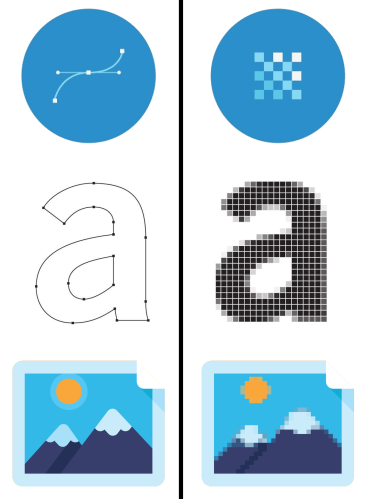
\includegraphics[width=0.45\textwidth,height=0.8\textheight,keepaspectratio]{figures/vector-raster.png}
 \caption{Imagem vetorial vs imagem rasterizada.}
 \label{fig-imgvr}
\end{figure}
\end{frame}

\begin{frame}[fragile]
\frametitle{Inserindo uma imagem em \LaTeX{}}
\begin{lstlisting}[language=tex, label=lst-figure, caption={Código para inserir uma figura em \LaTeX{}}, postbreak=\mbox{$\hookrightarrow$\space}, basicstyle=\fontsize{8}{10}\selectfont\ttfamily]
\begin{figure}[htbp]
 \centering
 \includegraphics[width=0.5\textwidth]{example-image-a}
 \caption{Legenda da figura.}
 \label{fig-img-a}
\end{figure}
\end{lstlisting}
\end{frame}



\begin{frame}
\frametitle{Tikz}
\begin{figure}[h]
\centering
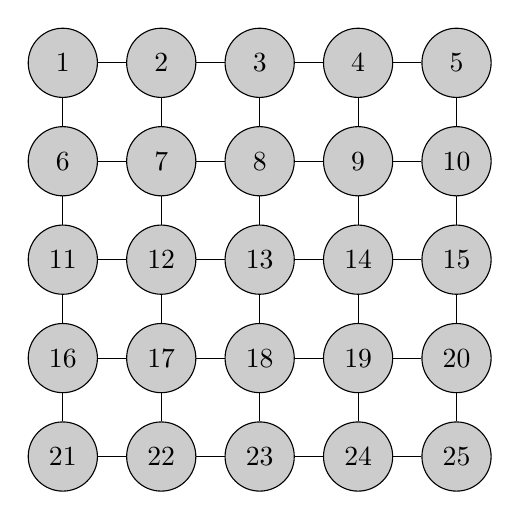
\begin{tikzpicture}[darkstyle/.style={circle,draw,fill=gray!40,minimum size=25}]
  \foreach \x in {0,...,4}
    \foreach \y in {0,...,4} 
       {\pgfmathtruncatemacro{\label}{\x - 5 *  \y +21}
       \node [darkstyle]  (\x\y) at (1.25*\x,1.25*\y) {\label};} 

  \foreach \x in {0,...,4}
    \foreach \y [count=\yi] in {0,...,3}  
      \draw (\x\y)--(\x\yi) (\y\x)--(\yi\x) ;
\end{tikzpicture}
\caption{Exemplo de utilização do Tikz.}
 \label{fig-tikz}
\end{figure}
\end{frame}


\begin{frame}[fragile]
\frametitle{Código exemplo Tikz}
\begin{lstlisting}[language=tex, label=lst-tikz, caption={Código utilizado para criar o exemplo em tikz.}, postbreak=\mbox{$\hookrightarrow$\space}, basicstyle=\fontsize{8}{10}\selectfont\ttfamily]
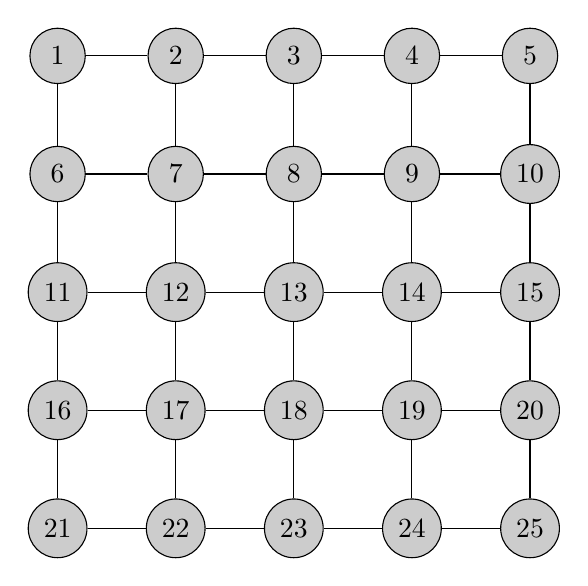
\begin{tikzpicture}[darkstyle/.style={circle,draw,fill=gray!40,minimum size=20}]
 \foreach \x in {0,...,4}
   \foreach \y in {0,...,4} 
      {\pgfmathtruncatemacro{\label}{\x - 5 *  \y +21}
      \node [darkstyle]  (\x\y) at (1.5*\x,1.5*\y) {\label};} 

 \foreach \x in {0,...,4}
   \foreach \y [count=\yi] in {0,...,3}  
     \draw (\x\y)--(\x\yi) (\y\x)--(\yi\x) ;
\end{tikzpicture}
\end{lstlisting}
\end{frame}


